\section{Appendix}
\begin{figure}[h]
  \centering
  \resizebox{.5\textwidth}{!}{% GNUPLOT: LaTeX picture with Postscript
\begingroup
  \makeatletter
  \providecommand\color[2][]{%
    \GenericError{(gnuplot) \space\space\space\@spaces}{%
      Package color not loaded in conjunction with
      terminal option `colourtext'%
    }{See the gnuplot documentation for explanation.%
    }{Either use 'blacktext' in gnuplot or load the package
      color.sty in LaTeX.}%
    \renewcommand\color[2][]{}%
  }%
  \providecommand\includegraphics[2][]{%
    \GenericError{(gnuplot) \space\space\space\@spaces}{%
      Package graphicx or graphics not loaded%
    }{See the gnuplot documentation for explanation.%
    }{The gnuplot epslatex terminal needs graphicx.sty or graphics.sty.}%
    \renewcommand\includegraphics[2][]{}%
  }%
  \providecommand\rotatebox[2]{#2}%
  \@ifundefined{ifGPcolor}{%
    \newif\ifGPcolor
    \GPcolortrue
  }{}%
  \@ifundefined{ifGPblacktext}{%
    \newif\ifGPblacktext
    \GPblacktexttrue
  }{}%
  % define a \g@addto@macro without @ in the name:
  \let\gplgaddtomacro\g@addto@macro
  % define empty templates for all commands taking text:
  \gdef\gplbacktext{}%
  \gdef\gplfronttext{}%
  \makeatother
  \ifGPblacktext
    % no textcolor at all
    \def\colorrgb#1{}%
    \def\colorgray#1{}%
  \else
    % gray or color?
    \ifGPcolor
      \def\colorrgb#1{\color[rgb]{#1}}%
      \def\colorgray#1{\color[gray]{#1}}%
      \expandafter\def\csname LTw\endcsname{\color{white}}%
      \expandafter\def\csname LTb\endcsname{\color{black}}%
      \expandafter\def\csname LTa\endcsname{\color{black}}%
      \expandafter\def\csname LT0\endcsname{\color[rgb]{1,0,0}}%
      \expandafter\def\csname LT1\endcsname{\color[rgb]{0,1,0}}%
      \expandafter\def\csname LT2\endcsname{\color[rgb]{0,0,1}}%
      \expandafter\def\csname LT3\endcsname{\color[rgb]{1,0,1}}%
      \expandafter\def\csname LT4\endcsname{\color[rgb]{0,1,1}}%
      \expandafter\def\csname LT5\endcsname{\color[rgb]{1,1,0}}%
      \expandafter\def\csname LT6\endcsname{\color[rgb]{0,0,0}}%
      \expandafter\def\csname LT7\endcsname{\color[rgb]{1,0.3,0}}%
      \expandafter\def\csname LT8\endcsname{\color[rgb]{0.5,0.5,0.5}}%
    \else
      % gray
      \def\colorrgb#1{\color{black}}%
      \def\colorgray#1{\color[gray]{#1}}%
      \expandafter\def\csname LTw\endcsname{\color{white}}%
      \expandafter\def\csname LTb\endcsname{\color{black}}%
      \expandafter\def\csname LTa\endcsname{\color{black}}%
      \expandafter\def\csname LT0\endcsname{\color{black}}%
      \expandafter\def\csname LT1\endcsname{\color{black}}%
      \expandafter\def\csname LT2\endcsname{\color{black}}%
      \expandafter\def\csname LT3\endcsname{\color{black}}%
      \expandafter\def\csname LT4\endcsname{\color{black}}%
      \expandafter\def\csname LT5\endcsname{\color{black}}%
      \expandafter\def\csname LT6\endcsname{\color{black}}%
      \expandafter\def\csname LT7\endcsname{\color{black}}%
      \expandafter\def\csname LT8\endcsname{\color{black}}%
    \fi
  \fi
    \setlength{\unitlength}{0.0500bp}%
    \ifx\gptboxheight\undefined%
      \newlength{\gptboxheight}%
      \newlength{\gptboxwidth}%
      \newsavebox{\gptboxtext}%
    \fi%
    \setlength{\fboxrule}{0.5pt}%
    \setlength{\fboxsep}{1pt}%
    \definecolor{tbcol}{rgb}{1,1,1}%
\begin{picture}(7200.00,4320.00)%
    \gplgaddtomacro\gplbacktext{%
      \csname LTb\endcsname%%
      \put(1123,619){\makebox(0,0)[r]{\strut{}200\cdot10^{-3}}}%
      \csname LTb\endcsname%%
      \put(1123,1006){\makebox(0,0)[r]{\strut{}300\cdot10^{-3}}}%
      \csname LTb\endcsname%%
      \put(1123,1394){\makebox(0,0)[r]{\strut{}400\cdot10^{-3}}}%
      \csname LTb\endcsname%%
      \put(1123,1781){\makebox(0,0)[r]{\strut{}500\cdot10^{-3}}}%
      \csname LTb\endcsname%%
      \put(1123,2169){\makebox(0,0)[r]{\strut{}600\cdot10^{-3}}}%
      \csname LTb\endcsname%%
      \put(1123,2556){\makebox(0,0)[r]{\strut{}700\cdot10^{-3}}}%
      \csname LTb\endcsname%%
      \put(1123,2944){\makebox(0,0)[r]{\strut{}800\cdot10^{-3}}}%
      \csname LTb\endcsname%%
      \put(1123,3331){\makebox(0,0)[r]{\strut{}900\cdot10^{-3}}}%
      \csname LTb\endcsname%%
      \put(1123,3719){\makebox(0,0)[r]{\strut{}1\cdot10^{0}}}%
      \csname LTb\endcsname%%
      \put(1221,425){\makebox(0,0){\strut{}$0$}}%
      \csname LTb\endcsname%%
      \put(1929,425){\makebox(0,0){\strut{}$100$}}%
      \csname LTb\endcsname%%
      \put(2637,425){\makebox(0,0){\strut{}$200$}}%
      \csname LTb\endcsname%%
      \put(3345,425){\makebox(0,0){\strut{}$300$}}%
      \csname LTb\endcsname%%
      \put(4053,425){\makebox(0,0){\strut{}$400$}}%
      \csname LTb\endcsname%%
      \put(4761,425){\makebox(0,0){\strut{}$500$}}%
      \csname LTb\endcsname%%
      \put(5470,425){\makebox(0,0){\strut{}$600$}}%
      \csname LTb\endcsname%%
      \put(6178,425){\makebox(0,0){\strut{}$700$}}%
      \csname LTb\endcsname%%
      \put(6886,425){\makebox(0,0){\strut{}$800$}}%
    }%
    \gplgaddtomacro\gplfronttext{%
      \csname LTb\endcsname%%
      \put(6123,3545){\makebox(0,0)[r]{\strut{}109358-G0}}%
      \csname LTb\endcsname%%
      \put(6123,3351){\makebox(0,0)[r]{\strut{}Kalibrationslampe}}%
      \csname LTb\endcsname%%
      \put(170,2169){\rotatebox{-270.00}{\makebox(0,0){\strut{}Amplitude$/\textrm{a.u.}$}}}%
      \csname LTb\endcsname%%
      \put(4053,135){\makebox(0,0){\strut{}Pixelkoordinate$/\textrm{Pixel}$}}%
      \csname LTb\endcsname%%
      \put(4053,4009){\makebox(0,0){\strut{}Spektrum}}%
    }%
    \gplbacktext
    \put(0,0){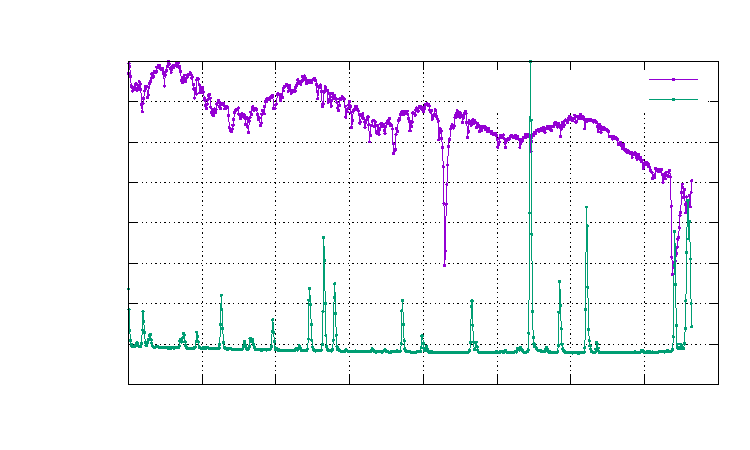
\includegraphics[width={360.00bp},height={216.00bp}]{109358-G0_data}}%
    \gplfronttext
  \end{picture}%
\endgroup
}
  \caption{}
\end{figure}
\begin{figure}[h]
  \centering
  \resizebox{.5\textwidth}{!}{% GNUPLOT: LaTeX picture with Postscript
\begingroup
  \makeatletter
  \providecommand\color[2][]{%
    \GenericError{(gnuplot) \space\space\space\@spaces}{%
      Package color not loaded in conjunction with
      terminal option `colourtext'%
    }{See the gnuplot documentation for explanation.%
    }{Either use 'blacktext' in gnuplot or load the package
      color.sty in LaTeX.}%
    \renewcommand\color[2][]{}%
  }%
  \providecommand\includegraphics[2][]{%
    \GenericError{(gnuplot) \space\space\space\@spaces}{%
      Package graphicx or graphics not loaded%
    }{See the gnuplot documentation for explanation.%
    }{The gnuplot epslatex terminal needs graphicx.sty or graphics.sty.}%
    \renewcommand\includegraphics[2][]{}%
  }%
  \providecommand\rotatebox[2]{#2}%
  \@ifundefined{ifGPcolor}{%
    \newif\ifGPcolor
    \GPcolortrue
  }{}%
  \@ifundefined{ifGPblacktext}{%
    \newif\ifGPblacktext
    \GPblacktexttrue
  }{}%
  % define a \g@addto@macro without @ in the name:
  \let\gplgaddtomacro\g@addto@macro
  % define empty templates for all commands taking text:
  \gdef\gplbacktext{}%
  \gdef\gplfronttext{}%
  \makeatother
  \ifGPblacktext
    % no textcolor at all
    \def\colorrgb#1{}%
    \def\colorgray#1{}%
  \else
    % gray or color?
    \ifGPcolor
      \def\colorrgb#1{\color[rgb]{#1}}%
      \def\colorgray#1{\color[gray]{#1}}%
      \expandafter\def\csname LTw\endcsname{\color{white}}%
      \expandafter\def\csname LTb\endcsname{\color{black}}%
      \expandafter\def\csname LTa\endcsname{\color{black}}%
      \expandafter\def\csname LT0\endcsname{\color[rgb]{1,0,0}}%
      \expandafter\def\csname LT1\endcsname{\color[rgb]{0,1,0}}%
      \expandafter\def\csname LT2\endcsname{\color[rgb]{0,0,1}}%
      \expandafter\def\csname LT3\endcsname{\color[rgb]{1,0,1}}%
      \expandafter\def\csname LT4\endcsname{\color[rgb]{0,1,1}}%
      \expandafter\def\csname LT5\endcsname{\color[rgb]{1,1,0}}%
      \expandafter\def\csname LT6\endcsname{\color[rgb]{0,0,0}}%
      \expandafter\def\csname LT7\endcsname{\color[rgb]{1,0.3,0}}%
      \expandafter\def\csname LT8\endcsname{\color[rgb]{0.5,0.5,0.5}}%
    \else
      % gray
      \def\colorrgb#1{\color{black}}%
      \def\colorgray#1{\color[gray]{#1}}%
      \expandafter\def\csname LTw\endcsname{\color{white}}%
      \expandafter\def\csname LTb\endcsname{\color{black}}%
      \expandafter\def\csname LTa\endcsname{\color{black}}%
      \expandafter\def\csname LT0\endcsname{\color{black}}%
      \expandafter\def\csname LT1\endcsname{\color{black}}%
      \expandafter\def\csname LT2\endcsname{\color{black}}%
      \expandafter\def\csname LT3\endcsname{\color{black}}%
      \expandafter\def\csname LT4\endcsname{\color{black}}%
      \expandafter\def\csname LT5\endcsname{\color{black}}%
      \expandafter\def\csname LT6\endcsname{\color{black}}%
      \expandafter\def\csname LT7\endcsname{\color{black}}%
      \expandafter\def\csname LT8\endcsname{\color{black}}%
    \fi
  \fi
    \setlength{\unitlength}{0.0500bp}%
    \ifx\gptboxheight\undefined%
      \newlength{\gptboxheight}%
      \newlength{\gptboxwidth}%
      \newsavebox{\gptboxtext}%
    \fi%
    \setlength{\fboxrule}{0.5pt}%
    \setlength{\fboxsep}{1pt}%
    \definecolor{tbcol}{rgb}{1,1,1}%
\begin{picture}(7200.00,4320.00)%
    \gplgaddtomacro\gplbacktext{%
      \csname LTb\endcsname%%
      \put(1025,619){\makebox(0,0)[r]{\strut{}$70\cdot10^{3}$}}%
      \csname LTb\endcsname%%
      \put(1025,1062){\makebox(0,0)[r]{\strut{}$80\cdot10^{3}$}}%
      \csname LTb\endcsname%%
      \put(1025,1505){\makebox(0,0)[r]{\strut{}$90\cdot10^{3}$}}%
      \csname LTb\endcsname%%
      \put(1025,1947){\makebox(0,0)[r]{\strut{}$100\cdot10^{3}$}}%
      \csname LTb\endcsname%%
      \put(1025,2390){\makebox(0,0)[r]{\strut{}$110\cdot10^{3}$}}%
      \csname LTb\endcsname%%
      \put(1025,2833){\makebox(0,0)[r]{\strut{}$120\cdot10^{3}$}}%
      \csname LTb\endcsname%%
      \put(1025,3276){\makebox(0,0)[r]{\strut{}$130\cdot10^{3}$}}%
      \csname LTb\endcsname%%
      \put(1025,3719){\makebox(0,0)[r]{\strut{}$140\cdot10^{3}$}}%
      \csname LTb\endcsname%%
      \put(2276,425){\makebox(0,0){\strut{}$650\cdot10^{-9}$}}%
      \csname LTb\endcsname%%
      \put(3716,425){\makebox(0,0){\strut{}$655\cdot10^{-9}$}}%
      \csname LTb\endcsname%%
      \put(5157,425){\makebox(0,0){\strut{}$660\cdot10^{-9}$}}%
      \csname LTb\endcsname%%
      \put(6598,425){\makebox(0,0){\strut{}$665\cdot10^{-9}$}}%
    }%
    \gplgaddtomacro\gplfronttext{%
      \csname LTb\endcsname%%
      \put(170,2169){\rotatebox{-270}{\makebox(0,0){\strut{}Amplitude$/\textrm{a.u.}$}}}%
      \csname LTb\endcsname%%
      \put(4004,135){\makebox(0,0){\strut{}Wellenlänge $\lambda/\SI{}{m}$}}%
      \csname LTb\endcsname%%
      \put(6123,986){\makebox(0,0)[r]{\strut{}Datenpunkte}}%
      \csname LTb\endcsname%%
      \put(6123,793){\makebox(0,0)[r]{\strut{}Anpassung $G_\text{f}(x)$}}%
      \csname LTb\endcsname%%
      \put(4004,4009){\makebox(0,0){\strut{}H$\alpha$(\SI{656}{nm})-Linie von 109358-G0 mit $\chi^2/\textrm{ddof}=\SI{1.16E+01}{}$}}%
    }%
    \gplbacktext
    \put(0,0){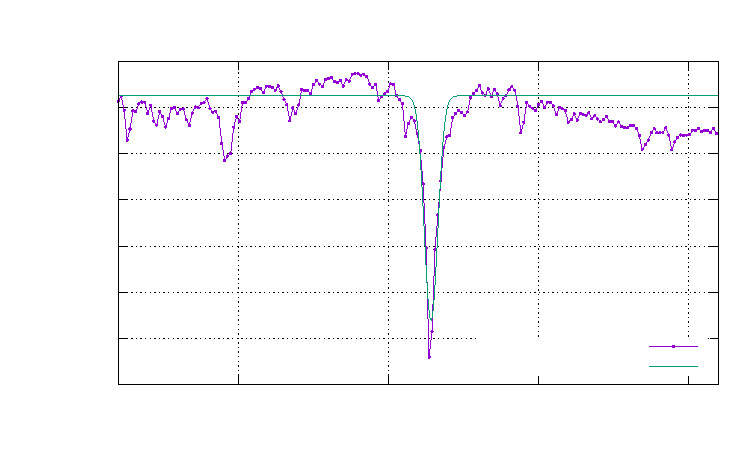
\includegraphics[width={360.00bp},height={216.00bp}]{109358-G0_gauss}}%
    \gplfronttext
  \end{picture}%
\endgroup
}
  \caption{}
\end{figure}
\begin{figure}[h]
  \centering
  \resizebox{.5\textwidth}{!}{% GNUPLOT: LaTeX picture with Postscript
\begingroup
  \makeatletter
  \providecommand\color[2][]{%
    \GenericError{(gnuplot) \space\space\space\@spaces}{%
      Package color not loaded in conjunction with
      terminal option `colourtext'%
    }{See the gnuplot documentation for explanation.%
    }{Either use 'blacktext' in gnuplot or load the package
      color.sty in LaTeX.}%
    \renewcommand\color[2][]{}%
  }%
  \providecommand\includegraphics[2][]{%
    \GenericError{(gnuplot) \space\space\space\@spaces}{%
      Package graphicx or graphics not loaded%
    }{See the gnuplot documentation for explanation.%
    }{The gnuplot epslatex terminal needs graphicx.sty or graphics.sty.}%
    \renewcommand\includegraphics[2][]{}%
  }%
  \providecommand\rotatebox[2]{#2}%
  \@ifundefined{ifGPcolor}{%
    \newif\ifGPcolor
    \GPcolortrue
  }{}%
  \@ifundefined{ifGPblacktext}{%
    \newif\ifGPblacktext
    \GPblacktexttrue
  }{}%
  % define a \g@addto@macro without @ in the name:
  \let\gplgaddtomacro\g@addto@macro
  % define empty templates for all commands taking text:
  \gdef\gplbacktext{}%
  \gdef\gplfronttext{}%
  \makeatother
  \ifGPblacktext
    % no textcolor at all
    \def\colorrgb#1{}%
    \def\colorgray#1{}%
  \else
    % gray or color?
    \ifGPcolor
      \def\colorrgb#1{\color[rgb]{#1}}%
      \def\colorgray#1{\color[gray]{#1}}%
      \expandafter\def\csname LTw\endcsname{\color{white}}%
      \expandafter\def\csname LTb\endcsname{\color{black}}%
      \expandafter\def\csname LTa\endcsname{\color{black}}%
      \expandafter\def\csname LT0\endcsname{\color[rgb]{1,0,0}}%
      \expandafter\def\csname LT1\endcsname{\color[rgb]{0,1,0}}%
      \expandafter\def\csname LT2\endcsname{\color[rgb]{0,0,1}}%
      \expandafter\def\csname LT3\endcsname{\color[rgb]{1,0,1}}%
      \expandafter\def\csname LT4\endcsname{\color[rgb]{0,1,1}}%
      \expandafter\def\csname LT5\endcsname{\color[rgb]{1,1,0}}%
      \expandafter\def\csname LT6\endcsname{\color[rgb]{0,0,0}}%
      \expandafter\def\csname LT7\endcsname{\color[rgb]{1,0.3,0}}%
      \expandafter\def\csname LT8\endcsname{\color[rgb]{0.5,0.5,0.5}}%
    \else
      % gray
      \def\colorrgb#1{\color{black}}%
      \def\colorgray#1{\color[gray]{#1}}%
      \expandafter\def\csname LTw\endcsname{\color{white}}%
      \expandafter\def\csname LTb\endcsname{\color{black}}%
      \expandafter\def\csname LTa\endcsname{\color{black}}%
      \expandafter\def\csname LT0\endcsname{\color{black}}%
      \expandafter\def\csname LT1\endcsname{\color{black}}%
      \expandafter\def\csname LT2\endcsname{\color{black}}%
      \expandafter\def\csname LT3\endcsname{\color{black}}%
      \expandafter\def\csname LT4\endcsname{\color{black}}%
      \expandafter\def\csname LT5\endcsname{\color{black}}%
      \expandafter\def\csname LT6\endcsname{\color{black}}%
      \expandafter\def\csname LT7\endcsname{\color{black}}%
      \expandafter\def\csname LT8\endcsname{\color{black}}%
    \fi
  \fi
    \setlength{\unitlength}{0.0500bp}%
    \ifx\gptboxheight\undefined%
      \newlength{\gptboxheight}%
      \newlength{\gptboxwidth}%
      \newsavebox{\gptboxtext}%
    \fi%
    \setlength{\fboxrule}{0.5pt}%
    \setlength{\fboxsep}{1pt}%
    \definecolor{tbcol}{rgb}{1,1,1}%
\begin{picture}(7200.00,4320.00)%
    \gplgaddtomacro\gplbacktext{%
      \csname LTb\endcsname%%
      \put(1123,619){\makebox(0,0)[r]{\strut{}635\cdot10^{-9}}}%
      \csname LTb\endcsname%%
      \put(1123,963){\makebox(0,0)[r]{\strut{}640\cdot10^{-9}}}%
      \csname LTb\endcsname%%
      \put(1123,1308){\makebox(0,0)[r]{\strut{}645\cdot10^{-9}}}%
      \csname LTb\endcsname%%
      \put(1123,1652){\makebox(0,0)[r]{\strut{}650\cdot10^{-9}}}%
      \csname LTb\endcsname%%
      \put(1123,1997){\makebox(0,0)[r]{\strut{}655\cdot10^{-9}}}%
      \csname LTb\endcsname%%
      \put(1123,2341){\makebox(0,0)[r]{\strut{}660\cdot10^{-9}}}%
      \csname LTb\endcsname%%
      \put(1123,2686){\makebox(0,0)[r]{\strut{}665\cdot10^{-9}}}%
      \csname LTb\endcsname%%
      \put(1123,3030){\makebox(0,0)[r]{\strut{}670\cdot10^{-9}}}%
      \csname LTb\endcsname%%
      \put(1123,3374){\makebox(0,0)[r]{\strut{}675\cdot10^{-9}}}%
      \csname LTb\endcsname%%
      \put(1123,3719){\makebox(0,0)[r]{\strut{}680\cdot10^{-9}}}%
      \csname LTb\endcsname%%
      \put(1221,425){\makebox(0,0){\strut{}$200$}}%
      \csname LTb\endcsname%%
      \put(1850,425){\makebox(0,0){\strut{}$250$}}%
      \csname LTb\endcsname%%
      \put(2480,425){\makebox(0,0){\strut{}$300$}}%
      \csname LTb\endcsname%%
      \put(3109,425){\makebox(0,0){\strut{}$350$}}%
      \csname LTb\endcsname%%
      \put(3739,425){\makebox(0,0){\strut{}$400$}}%
      \csname LTb\endcsname%%
      \put(4368,425){\makebox(0,0){\strut{}$450$}}%
      \csname LTb\endcsname%%
      \put(4997,425){\makebox(0,0){\strut{}$500$}}%
      \csname LTb\endcsname%%
      \put(5627,425){\makebox(0,0){\strut{}$550$}}%
      \csname LTb\endcsname%%
      \put(6256,425){\makebox(0,0){\strut{}$600$}}%
      \csname LTb\endcsname%%
      \put(6886,425){\makebox(0,0){\strut{}$650$}}%
    }%
    \gplgaddtomacro\gplfronttext{%
      \csname LTb\endcsname%%
      \put(6123,3545){\makebox(0,0)[r]{\strut{}Datenpunkte}}%
      \csname LTb\endcsname%%
      \put(6123,3351){\makebox(0,0)[r]{\strut{}Anpassung $\lambda_\text{f}(x)$}}%
      \csname LTb\endcsname%%
      \put(170,2169){\rotatebox{-270.00}{\makebox(0,0){\strut{}Wellenlänge $\lambda/\SI{}{m}$}}}%
      \csname LTb\endcsname%%
      \put(4053,135){\makebox(0,0){\strut{}Pixelkoordinate$/\textrm{Pixel}$}}%
      \csname LTb\endcsname%%
      \put(4053,4009){\makebox(0,0){\strut{}Kalibraiton des 109358-G0 Spektrums mit $\chi^2/\textrm{ddof}=\SI{3.03E-02}{}$}}%
    }%
    \gplbacktext
    \put(0,0){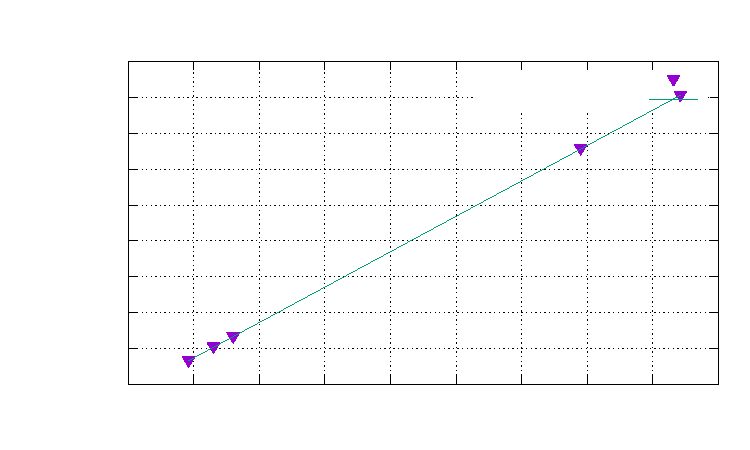
\includegraphics[width={360.00bp},height={216.00bp}]{109358-G0_kali}}%
    \gplfronttext
  \end{picture}%
\endgroup
}
  \caption{}
\end{figure}
\begin{figure}[h]
  \centering
  \resizebox{.5\textwidth}{!}{% GNUPLOT: LaTeX picture with Postscript
\begingroup
  \makeatletter
  \providecommand\color[2][]{%
    \GenericError{(gnuplot) \space\space\space\@spaces}{%
      Package color not loaded in conjunction with
      terminal option `colourtext'%
    }{See the gnuplot documentation for explanation.%
    }{Either use 'blacktext' in gnuplot or load the package
      color.sty in LaTeX.}%
    \renewcommand\color[2][]{}%
  }%
  \providecommand\includegraphics[2][]{%
    \GenericError{(gnuplot) \space\space\space\@spaces}{%
      Package graphicx or graphics not loaded%
    }{See the gnuplot documentation for explanation.%
    }{The gnuplot epslatex terminal needs graphicx.sty or graphics.sty.}%
    \renewcommand\includegraphics[2][]{}%
  }%
  \providecommand\rotatebox[2]{#2}%
  \@ifundefined{ifGPcolor}{%
    \newif\ifGPcolor
    \GPcolortrue
  }{}%
  \@ifundefined{ifGPblacktext}{%
    \newif\ifGPblacktext
    \GPblacktexttrue
  }{}%
  % define a \g@addto@macro without @ in the name:
  \let\gplgaddtomacro\g@addto@macro
  % define empty templates for all commands taking text:
  \gdef\gplbacktext{}%
  \gdef\gplfronttext{}%
  \makeatother
  \ifGPblacktext
    % no textcolor at all
    \def\colorrgb#1{}%
    \def\colorgray#1{}%
  \else
    % gray or color?
    \ifGPcolor
      \def\colorrgb#1{\color[rgb]{#1}}%
      \def\colorgray#1{\color[gray]{#1}}%
      \expandafter\def\csname LTw\endcsname{\color{white}}%
      \expandafter\def\csname LTb\endcsname{\color{black}}%
      \expandafter\def\csname LTa\endcsname{\color{black}}%
      \expandafter\def\csname LT0\endcsname{\color[rgb]{1,0,0}}%
      \expandafter\def\csname LT1\endcsname{\color[rgb]{0,1,0}}%
      \expandafter\def\csname LT2\endcsname{\color[rgb]{0,0,1}}%
      \expandafter\def\csname LT3\endcsname{\color[rgb]{1,0,1}}%
      \expandafter\def\csname LT4\endcsname{\color[rgb]{0,1,1}}%
      \expandafter\def\csname LT5\endcsname{\color[rgb]{1,1,0}}%
      \expandafter\def\csname LT6\endcsname{\color[rgb]{0,0,0}}%
      \expandafter\def\csname LT7\endcsname{\color[rgb]{1,0.3,0}}%
      \expandafter\def\csname LT8\endcsname{\color[rgb]{0.5,0.5,0.5}}%
    \else
      % gray
      \def\colorrgb#1{\color{black}}%
      \def\colorgray#1{\color[gray]{#1}}%
      \expandafter\def\csname LTw\endcsname{\color{white}}%
      \expandafter\def\csname LTb\endcsname{\color{black}}%
      \expandafter\def\csname LTa\endcsname{\color{black}}%
      \expandafter\def\csname LT0\endcsname{\color{black}}%
      \expandafter\def\csname LT1\endcsname{\color{black}}%
      \expandafter\def\csname LT2\endcsname{\color{black}}%
      \expandafter\def\csname LT3\endcsname{\color{black}}%
      \expandafter\def\csname LT4\endcsname{\color{black}}%
      \expandafter\def\csname LT5\endcsname{\color{black}}%
      \expandafter\def\csname LT6\endcsname{\color{black}}%
      \expandafter\def\csname LT7\endcsname{\color{black}}%
      \expandafter\def\csname LT8\endcsname{\color{black}}%
    \fi
  \fi
    \setlength{\unitlength}{0.0500bp}%
    \ifx\gptboxheight\undefined%
      \newlength{\gptboxheight}%
      \newlength{\gptboxwidth}%
      \newsavebox{\gptboxtext}%
    \fi%
    \setlength{\fboxrule}{0.5pt}%
    \setlength{\fboxsep}{1pt}%
    \definecolor{tbcol}{rgb}{1,1,1}%
\begin{picture}(7200.00,4320.00)%
    \gplgaddtomacro\gplbacktext{%
      \csname LTb\endcsname%%
      \put(1123,619){\makebox(0,0)[r]{\strut{}$200\cdot10^{-3}$}}%
      \csname LTb\endcsname%%
      \put(1123,1006){\makebox(0,0)[r]{\strut{}$300\cdot10^{-3}$}}%
      \csname LTb\endcsname%%
      \put(1123,1394){\makebox(0,0)[r]{\strut{}$400\cdot10^{-3}$}}%
      \csname LTb\endcsname%%
      \put(1123,1781){\makebox(0,0)[r]{\strut{}$500\cdot10^{-3}$}}%
      \csname LTb\endcsname%%
      \put(1123,2169){\makebox(0,0)[r]{\strut{}$600\cdot10^{-3}$}}%
      \csname LTb\endcsname%%
      \put(1123,2556){\makebox(0,0)[r]{\strut{}$700\cdot10^{-3}$}}%
      \csname LTb\endcsname%%
      \put(1123,2944){\makebox(0,0)[r]{\strut{}$800\cdot10^{-3}$}}%
      \csname LTb\endcsname%%
      \put(1123,3331){\makebox(0,0)[r]{\strut{}$900\cdot10^{-3}$}}%
      \csname LTb\endcsname%%
      \put(1123,3719){\makebox(0,0)[r]{\strut{}$1\cdot10^{0}$}}%
      \csname LTb\endcsname%%
      \put(1221,425){\makebox(0,0){\strut{}$0$}}%
      \csname LTb\endcsname%%
      \put(1929,425){\makebox(0,0){\strut{}$100$}}%
      \csname LTb\endcsname%%
      \put(2637,425){\makebox(0,0){\strut{}$200$}}%
      \csname LTb\endcsname%%
      \put(3345,425){\makebox(0,0){\strut{}$300$}}%
      \csname LTb\endcsname%%
      \put(4053,425){\makebox(0,0){\strut{}$400$}}%
      \csname LTb\endcsname%%
      \put(4761,425){\makebox(0,0){\strut{}$500$}}%
      \csname LTb\endcsname%%
      \put(5470,425){\makebox(0,0){\strut{}$600$}}%
      \csname LTb\endcsname%%
      \put(6178,425){\makebox(0,0){\strut{}$700$}}%
      \csname LTb\endcsname%%
      \put(6886,425){\makebox(0,0){\strut{}$800$}}%
    }%
    \gplgaddtomacro\gplfronttext{%
      \csname LTb\endcsname%%
      \put(170,2169){\rotatebox{-270}{\makebox(0,0){\strut{}Amplitude$/\textrm{a.u.}$}}}%
      \csname LTb\endcsname%%
      \put(4053,135){\makebox(0,0){\strut{}Pixelkoordinate$/\textrm{Pixel}$}}%
      \csname LTb\endcsname%%
      \put(6123,3545){\makebox(0,0)[r]{\strut{}134083-F5}}%
      \csname LTb\endcsname%%
      \put(6123,3351){\makebox(0,0)[r]{\strut{}Kalibrationslampe}}%
      \csname LTb\endcsname%%
      \put(4053,4009){\makebox(0,0){\strut{}Spektrum}}%
    }%
    \gplbacktext
    \put(0,0){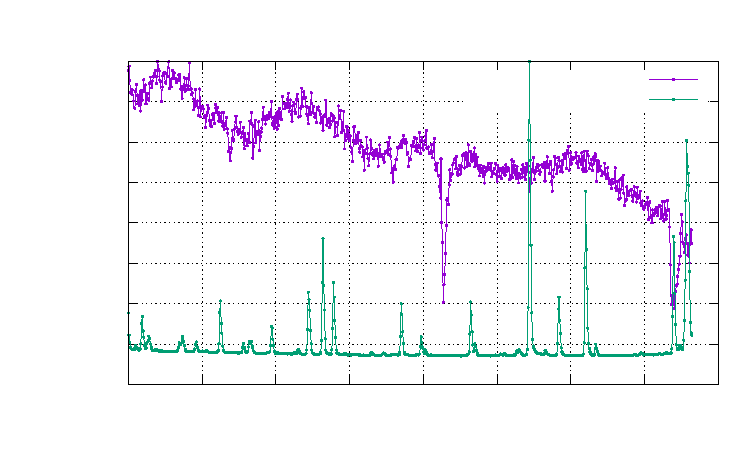
\includegraphics[width={360.00bp},height={216.00bp}]{134083-F5_data}}%
    \gplfronttext
  \end{picture}%
\endgroup
}
  \caption{}
\end{figure}
\begin{figure}[h]
  \centering
  \resizebox{.5\textwidth}{!}{% GNUPLOT: LaTeX picture with Postscript
\begingroup
  \makeatletter
  \providecommand\color[2][]{%
    \GenericError{(gnuplot) \space\space\space\@spaces}{%
      Package color not loaded in conjunction with
      terminal option `colourtext'%
    }{See the gnuplot documentation for explanation.%
    }{Either use 'blacktext' in gnuplot or load the package
      color.sty in LaTeX.}%
    \renewcommand\color[2][]{}%
  }%
  \providecommand\includegraphics[2][]{%
    \GenericError{(gnuplot) \space\space\space\@spaces}{%
      Package graphicx or graphics not loaded%
    }{See the gnuplot documentation for explanation.%
    }{The gnuplot epslatex terminal needs graphicx.sty or graphics.sty.}%
    \renewcommand\includegraphics[2][]{}%
  }%
  \providecommand\rotatebox[2]{#2}%
  \@ifundefined{ifGPcolor}{%
    \newif\ifGPcolor
    \GPcolortrue
  }{}%
  \@ifundefined{ifGPblacktext}{%
    \newif\ifGPblacktext
    \GPblacktexttrue
  }{}%
  % define a \g@addto@macro without @ in the name:
  \let\gplgaddtomacro\g@addto@macro
  % define empty templates for all commands taking text:
  \gdef\gplbacktext{}%
  \gdef\gplfronttext{}%
  \makeatother
  \ifGPblacktext
    % no textcolor at all
    \def\colorrgb#1{}%
    \def\colorgray#1{}%
  \else
    % gray or color?
    \ifGPcolor
      \def\colorrgb#1{\color[rgb]{#1}}%
      \def\colorgray#1{\color[gray]{#1}}%
      \expandafter\def\csname LTw\endcsname{\color{white}}%
      \expandafter\def\csname LTb\endcsname{\color{black}}%
      \expandafter\def\csname LTa\endcsname{\color{black}}%
      \expandafter\def\csname LT0\endcsname{\color[rgb]{1,0,0}}%
      \expandafter\def\csname LT1\endcsname{\color[rgb]{0,1,0}}%
      \expandafter\def\csname LT2\endcsname{\color[rgb]{0,0,1}}%
      \expandafter\def\csname LT3\endcsname{\color[rgb]{1,0,1}}%
      \expandafter\def\csname LT4\endcsname{\color[rgb]{0,1,1}}%
      \expandafter\def\csname LT5\endcsname{\color[rgb]{1,1,0}}%
      \expandafter\def\csname LT6\endcsname{\color[rgb]{0,0,0}}%
      \expandafter\def\csname LT7\endcsname{\color[rgb]{1,0.3,0}}%
      \expandafter\def\csname LT8\endcsname{\color[rgb]{0.5,0.5,0.5}}%
    \else
      % gray
      \def\colorrgb#1{\color{black}}%
      \def\colorgray#1{\color[gray]{#1}}%
      \expandafter\def\csname LTw\endcsname{\color{white}}%
      \expandafter\def\csname LTb\endcsname{\color{black}}%
      \expandafter\def\csname LTa\endcsname{\color{black}}%
      \expandafter\def\csname LT0\endcsname{\color{black}}%
      \expandafter\def\csname LT1\endcsname{\color{black}}%
      \expandafter\def\csname LT2\endcsname{\color{black}}%
      \expandafter\def\csname LT3\endcsname{\color{black}}%
      \expandafter\def\csname LT4\endcsname{\color{black}}%
      \expandafter\def\csname LT5\endcsname{\color{black}}%
      \expandafter\def\csname LT6\endcsname{\color{black}}%
      \expandafter\def\csname LT7\endcsname{\color{black}}%
      \expandafter\def\csname LT8\endcsname{\color{black}}%
    \fi
  \fi
    \setlength{\unitlength}{0.0500bp}%
    \ifx\gptboxheight\undefined%
      \newlength{\gptboxheight}%
      \newlength{\gptboxwidth}%
      \newsavebox{\gptboxtext}%
    \fi%
    \setlength{\fboxrule}{0.5pt}%
    \setlength{\fboxsep}{1pt}%
    \definecolor{tbcol}{rgb}{1,1,1}%
\begin{picture}(7200.00,4320.00)%
    \gplgaddtomacro\gplbacktext{%
      \csname LTb\endcsname%%
      \put(927,619){\makebox(0,0)[r]{\strut{}$9\cdot10^{3}$}}%
      \csname LTb\endcsname%%
      \put(927,929){\makebox(0,0)[r]{\strut{}$10\cdot10^{3}$}}%
      \csname LTb\endcsname%%
      \put(927,1239){\makebox(0,0)[r]{\strut{}$11\cdot10^{3}$}}%
      \csname LTb\endcsname%%
      \put(927,1549){\makebox(0,0)[r]{\strut{}$12\cdot10^{3}$}}%
      \csname LTb\endcsname%%
      \put(927,1859){\makebox(0,0)[r]{\strut{}$13\cdot10^{3}$}}%
      \csname LTb\endcsname%%
      \put(927,2169){\makebox(0,0)[r]{\strut{}$14\cdot10^{3}$}}%
      \csname LTb\endcsname%%
      \put(927,2479){\makebox(0,0)[r]{\strut{}$15\cdot10^{3}$}}%
      \csname LTb\endcsname%%
      \put(927,2789){\makebox(0,0)[r]{\strut{}$16\cdot10^{3}$}}%
      \csname LTb\endcsname%%
      \put(927,3099){\makebox(0,0)[r]{\strut{}$17\cdot10^{3}$}}%
      \csname LTb\endcsname%%
      \put(927,3409){\makebox(0,0)[r]{\strut{}$18\cdot10^{3}$}}%
      \csname LTb\endcsname%%
      \put(927,3719){\makebox(0,0)[r]{\strut{}$19\cdot10^{3}$}}%
      \csname LTb\endcsname%%
      \put(2197,425){\makebox(0,0){\strut{}$650\cdot10^{-9}$}}%
      \csname LTb\endcsname%%
      \put(3662,425){\makebox(0,0){\strut{}$655\cdot10^{-9}$}}%
      \csname LTb\endcsname%%
      \put(5128,425){\makebox(0,0){\strut{}$660\cdot10^{-9}$}}%
      \csname LTb\endcsname%%
      \put(6593,425){\makebox(0,0){\strut{}$665\cdot10^{-9}$}}%
    }%
    \gplgaddtomacro\gplfronttext{%
      \csname LTb\endcsname%%
      \put(170,2169){\rotatebox{-270}{\makebox(0,0){\strut{}Amplitude$/\textrm{a.u.}$}}}%
      \csname LTb\endcsname%%
      \put(3955,135){\makebox(0,0){\strut{}Wellenlänge $\lambda/\SI{}{m}$}}%
      \csname LTb\endcsname%%
      \put(6123,986){\makebox(0,0)[r]{\strut{}Datenpunkte}}%
      \csname LTb\endcsname%%
      \put(6123,793){\makebox(0,0)[r]{\strut{}Anpassung $G_\text{f}(x)$}}%
      \csname LTb\endcsname%%
      \put(3955,4009){\makebox(0,0){\strut{}H$\alpha$(\SI{656}{nm})-Linie von 134083-F5 mit $\chi^2/\textrm{ddof}=\SI{5.18E-01}{}$}}%
    }%
    \gplbacktext
    \put(0,0){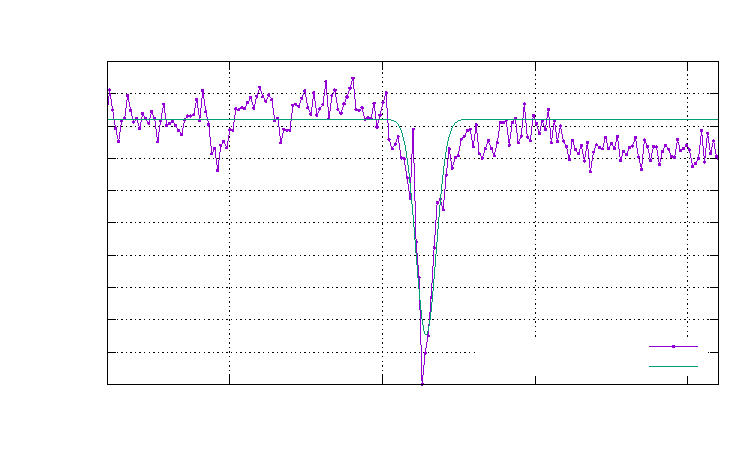
\includegraphics[width={360.00bp},height={216.00bp}]{134083-F5_gauss}}%
    \gplfronttext
  \end{picture}%
\endgroup
}
  \caption{}
\end{figure}
\begin{figure}[h]
  \centering
  \resizebox{.5\textwidth}{!}{% GNUPLOT: LaTeX picture with Postscript
\begingroup
  \makeatletter
  \providecommand\color[2][]{%
    \GenericError{(gnuplot) \space\space\space\@spaces}{%
      Package color not loaded in conjunction with
      terminal option `colourtext'%
    }{See the gnuplot documentation for explanation.%
    }{Either use 'blacktext' in gnuplot or load the package
      color.sty in LaTeX.}%
    \renewcommand\color[2][]{}%
  }%
  \providecommand\includegraphics[2][]{%
    \GenericError{(gnuplot) \space\space\space\@spaces}{%
      Package graphicx or graphics not loaded%
    }{See the gnuplot documentation for explanation.%
    }{The gnuplot epslatex terminal needs graphicx.sty or graphics.sty.}%
    \renewcommand\includegraphics[2][]{}%
  }%
  \providecommand\rotatebox[2]{#2}%
  \@ifundefined{ifGPcolor}{%
    \newif\ifGPcolor
    \GPcolortrue
  }{}%
  \@ifundefined{ifGPblacktext}{%
    \newif\ifGPblacktext
    \GPblacktexttrue
  }{}%
  % define a \g@addto@macro without @ in the name:
  \let\gplgaddtomacro\g@addto@macro
  % define empty templates for all commands taking text:
  \gdef\gplbacktext{}%
  \gdef\gplfronttext{}%
  \makeatother
  \ifGPblacktext
    % no textcolor at all
    \def\colorrgb#1{}%
    \def\colorgray#1{}%
  \else
    % gray or color?
    \ifGPcolor
      \def\colorrgb#1{\color[rgb]{#1}}%
      \def\colorgray#1{\color[gray]{#1}}%
      \expandafter\def\csname LTw\endcsname{\color{white}}%
      \expandafter\def\csname LTb\endcsname{\color{black}}%
      \expandafter\def\csname LTa\endcsname{\color{black}}%
      \expandafter\def\csname LT0\endcsname{\color[rgb]{1,0,0}}%
      \expandafter\def\csname LT1\endcsname{\color[rgb]{0,1,0}}%
      \expandafter\def\csname LT2\endcsname{\color[rgb]{0,0,1}}%
      \expandafter\def\csname LT3\endcsname{\color[rgb]{1,0,1}}%
      \expandafter\def\csname LT4\endcsname{\color[rgb]{0,1,1}}%
      \expandafter\def\csname LT5\endcsname{\color[rgb]{1,1,0}}%
      \expandafter\def\csname LT6\endcsname{\color[rgb]{0,0,0}}%
      \expandafter\def\csname LT7\endcsname{\color[rgb]{1,0.3,0}}%
      \expandafter\def\csname LT8\endcsname{\color[rgb]{0.5,0.5,0.5}}%
    \else
      % gray
      \def\colorrgb#1{\color{black}}%
      \def\colorgray#1{\color[gray]{#1}}%
      \expandafter\def\csname LTw\endcsname{\color{white}}%
      \expandafter\def\csname LTb\endcsname{\color{black}}%
      \expandafter\def\csname LTa\endcsname{\color{black}}%
      \expandafter\def\csname LT0\endcsname{\color{black}}%
      \expandafter\def\csname LT1\endcsname{\color{black}}%
      \expandafter\def\csname LT2\endcsname{\color{black}}%
      \expandafter\def\csname LT3\endcsname{\color{black}}%
      \expandafter\def\csname LT4\endcsname{\color{black}}%
      \expandafter\def\csname LT5\endcsname{\color{black}}%
      \expandafter\def\csname LT6\endcsname{\color{black}}%
      \expandafter\def\csname LT7\endcsname{\color{black}}%
      \expandafter\def\csname LT8\endcsname{\color{black}}%
    \fi
  \fi
    \setlength{\unitlength}{0.0500bp}%
    \ifx\gptboxheight\undefined%
      \newlength{\gptboxheight}%
      \newlength{\gptboxwidth}%
      \newsavebox{\gptboxtext}%
    \fi%
    \setlength{\fboxrule}{0.5pt}%
    \setlength{\fboxsep}{1pt}%
    \definecolor{tbcol}{rgb}{1,1,1}%
\begin{picture}(7200.00,4320.00)%
    \gplgaddtomacro\gplbacktext{%
      \csname LTb\endcsname%%
      \put(1123,619){\makebox(0,0)[r]{\strut{}635\cdot10^{-9}}}%
      \csname LTb\endcsname%%
      \put(1123,963){\makebox(0,0)[r]{\strut{}640\cdot10^{-9}}}%
      \csname LTb\endcsname%%
      \put(1123,1308){\makebox(0,0)[r]{\strut{}645\cdot10^{-9}}}%
      \csname LTb\endcsname%%
      \put(1123,1652){\makebox(0,0)[r]{\strut{}650\cdot10^{-9}}}%
      \csname LTb\endcsname%%
      \put(1123,1997){\makebox(0,0)[r]{\strut{}655\cdot10^{-9}}}%
      \csname LTb\endcsname%%
      \put(1123,2341){\makebox(0,0)[r]{\strut{}660\cdot10^{-9}}}%
      \csname LTb\endcsname%%
      \put(1123,2686){\makebox(0,0)[r]{\strut{}665\cdot10^{-9}}}%
      \csname LTb\endcsname%%
      \put(1123,3030){\makebox(0,0)[r]{\strut{}670\cdot10^{-9}}}%
      \csname LTb\endcsname%%
      \put(1123,3374){\makebox(0,0)[r]{\strut{}675\cdot10^{-9}}}%
      \csname LTb\endcsname%%
      \put(1123,3719){\makebox(0,0)[r]{\strut{}680\cdot10^{-9}}}%
      \csname LTb\endcsname%%
      \put(1221,425){\makebox(0,0){\strut{}$200$}}%
      \csname LTb\endcsname%%
      \put(1850,425){\makebox(0,0){\strut{}$250$}}%
      \csname LTb\endcsname%%
      \put(2480,425){\makebox(0,0){\strut{}$300$}}%
      \csname LTb\endcsname%%
      \put(3109,425){\makebox(0,0){\strut{}$350$}}%
      \csname LTb\endcsname%%
      \put(3739,425){\makebox(0,0){\strut{}$400$}}%
      \csname LTb\endcsname%%
      \put(4368,425){\makebox(0,0){\strut{}$450$}}%
      \csname LTb\endcsname%%
      \put(4997,425){\makebox(0,0){\strut{}$500$}}%
      \csname LTb\endcsname%%
      \put(5627,425){\makebox(0,0){\strut{}$550$}}%
      \csname LTb\endcsname%%
      \put(6256,425){\makebox(0,0){\strut{}$600$}}%
      \csname LTb\endcsname%%
      \put(6886,425){\makebox(0,0){\strut{}$650$}}%
    }%
    \gplgaddtomacro\gplfronttext{%
      \csname LTb\endcsname%%
      \put(6123,3545){\makebox(0,0)[r]{\strut{}Datenpunkte}}%
      \csname LTb\endcsname%%
      \put(6123,3351){\makebox(0,0)[r]{\strut{}Anpassung $\lambda_\text{f}(x)$}}%
      \csname LTb\endcsname%%
      \put(170,2169){\rotatebox{-270.00}{\makebox(0,0){\strut{}Wellenlänge $\lambda/\SI{}{m}$}}}%
      \csname LTb\endcsname%%
      \put(4053,135){\makebox(0,0){\strut{}Pixelkoordinate$/\textrm{Pixel}$}}%
      \csname LTb\endcsname%%
      \put(4053,4009){\makebox(0,0){\strut{}Kalibraiton des 134083-F5 Spektrums mit $\chi^2/\textrm{ddof}=\SI{1.45E-02}{}$}}%
    }%
    \gplbacktext
    \put(0,0){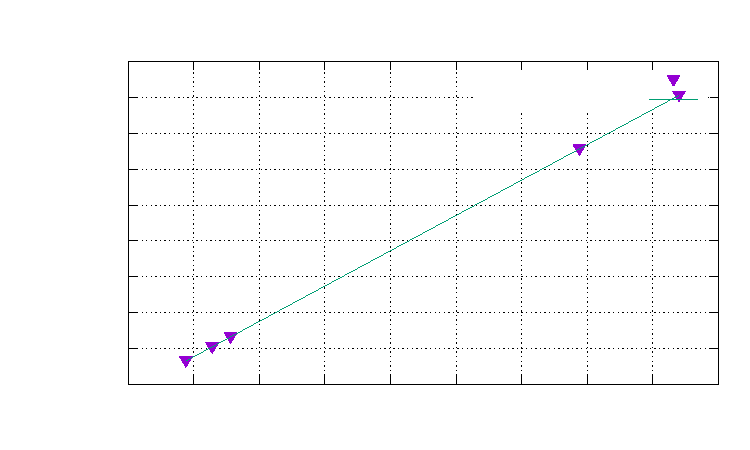
\includegraphics[width={360.00bp},height={216.00bp}]{134083-F5_kali}}%
    \gplfronttext
  \end{picture}%
\endgroup
}
  \caption{}
\end{figure}
\begin{figure}[h]
  \centering
  \resizebox{.5\textwidth}{!}{% GNUPLOT: LaTeX picture with Postscript
\begingroup
  \makeatletter
  \providecommand\color[2][]{%
    \GenericError{(gnuplot) \space\space\space\@spaces}{%
      Package color not loaded in conjunction with
      terminal option `colourtext'%
    }{See the gnuplot documentation for explanation.%
    }{Either use 'blacktext' in gnuplot or load the package
      color.sty in LaTeX.}%
    \renewcommand\color[2][]{}%
  }%
  \providecommand\includegraphics[2][]{%
    \GenericError{(gnuplot) \space\space\space\@spaces}{%
      Package graphicx or graphics not loaded%
    }{See the gnuplot documentation for explanation.%
    }{The gnuplot epslatex terminal needs graphicx.sty or graphics.sty.}%
    \renewcommand\includegraphics[2][]{}%
  }%
  \providecommand\rotatebox[2]{#2}%
  \@ifundefined{ifGPcolor}{%
    \newif\ifGPcolor
    \GPcolortrue
  }{}%
  \@ifundefined{ifGPblacktext}{%
    \newif\ifGPblacktext
    \GPblacktexttrue
  }{}%
  % define a \g@addto@macro without @ in the name:
  \let\gplgaddtomacro\g@addto@macro
  % define empty templates for all commands taking text:
  \gdef\gplbacktext{}%
  \gdef\gplfronttext{}%
  \makeatother
  \ifGPblacktext
    % no textcolor at all
    \def\colorrgb#1{}%
    \def\colorgray#1{}%
  \else
    % gray or color?
    \ifGPcolor
      \def\colorrgb#1{\color[rgb]{#1}}%
      \def\colorgray#1{\color[gray]{#1}}%
      \expandafter\def\csname LTw\endcsname{\color{white}}%
      \expandafter\def\csname LTb\endcsname{\color{black}}%
      \expandafter\def\csname LTa\endcsname{\color{black}}%
      \expandafter\def\csname LT0\endcsname{\color[rgb]{1,0,0}}%
      \expandafter\def\csname LT1\endcsname{\color[rgb]{0,1,0}}%
      \expandafter\def\csname LT2\endcsname{\color[rgb]{0,0,1}}%
      \expandafter\def\csname LT3\endcsname{\color[rgb]{1,0,1}}%
      \expandafter\def\csname LT4\endcsname{\color[rgb]{0,1,1}}%
      \expandafter\def\csname LT5\endcsname{\color[rgb]{1,1,0}}%
      \expandafter\def\csname LT6\endcsname{\color[rgb]{0,0,0}}%
      \expandafter\def\csname LT7\endcsname{\color[rgb]{1,0.3,0}}%
      \expandafter\def\csname LT8\endcsname{\color[rgb]{0.5,0.5,0.5}}%
    \else
      % gray
      \def\colorrgb#1{\color{black}}%
      \def\colorgray#1{\color[gray]{#1}}%
      \expandafter\def\csname LTw\endcsname{\color{white}}%
      \expandafter\def\csname LTb\endcsname{\color{black}}%
      \expandafter\def\csname LTa\endcsname{\color{black}}%
      \expandafter\def\csname LT0\endcsname{\color{black}}%
      \expandafter\def\csname LT1\endcsname{\color{black}}%
      \expandafter\def\csname LT2\endcsname{\color{black}}%
      \expandafter\def\csname LT3\endcsname{\color{black}}%
      \expandafter\def\csname LT4\endcsname{\color{black}}%
      \expandafter\def\csname LT5\endcsname{\color{black}}%
      \expandafter\def\csname LT6\endcsname{\color{black}}%
      \expandafter\def\csname LT7\endcsname{\color{black}}%
      \expandafter\def\csname LT8\endcsname{\color{black}}%
    \fi
  \fi
    \setlength{\unitlength}{0.0500bp}%
    \ifx\gptboxheight\undefined%
      \newlength{\gptboxheight}%
      \newlength{\gptboxwidth}%
      \newsavebox{\gptboxtext}%
    \fi%
    \setlength{\fboxrule}{0.5pt}%
    \setlength{\fboxsep}{1pt}%
    \definecolor{tbcol}{rgb}{1,1,1}%
\begin{picture}(7200.00,4320.00)%
    \gplgaddtomacro\gplbacktext{%
      \csname LTb\endcsname%%
      \put(1123,619){\makebox(0,0)[r]{\strut{}$400\cdot10^{-3}$}}%
      \csname LTb\endcsname%%
      \put(1123,1135){\makebox(0,0)[r]{\strut{}$500\cdot10^{-3}$}}%
      \csname LTb\endcsname%%
      \put(1123,1652){\makebox(0,0)[r]{\strut{}$600\cdot10^{-3}$}}%
      \csname LTb\endcsname%%
      \put(1123,2169){\makebox(0,0)[r]{\strut{}$700\cdot10^{-3}$}}%
      \csname LTb\endcsname%%
      \put(1123,2686){\makebox(0,0)[r]{\strut{}$800\cdot10^{-3}$}}%
      \csname LTb\endcsname%%
      \put(1123,3202){\makebox(0,0)[r]{\strut{}$900\cdot10^{-3}$}}%
      \csname LTb\endcsname%%
      \put(1123,3719){\makebox(0,0)[r]{\strut{}$1\cdot10^{0}$}}%
      \csname LTb\endcsname%%
      \put(1221,425){\makebox(0,0){\strut{}$0$}}%
      \csname LTb\endcsname%%
      \put(1929,425){\makebox(0,0){\strut{}$100$}}%
      \csname LTb\endcsname%%
      \put(2637,425){\makebox(0,0){\strut{}$200$}}%
      \csname LTb\endcsname%%
      \put(3345,425){\makebox(0,0){\strut{}$300$}}%
      \csname LTb\endcsname%%
      \put(4053,425){\makebox(0,0){\strut{}$400$}}%
      \csname LTb\endcsname%%
      \put(4761,425){\makebox(0,0){\strut{}$500$}}%
      \csname LTb\endcsname%%
      \put(5470,425){\makebox(0,0){\strut{}$600$}}%
      \csname LTb\endcsname%%
      \put(6178,425){\makebox(0,0){\strut{}$700$}}%
      \csname LTb\endcsname%%
      \put(6886,425){\makebox(0,0){\strut{}$800$}}%
    }%
    \gplgaddtomacro\gplfronttext{%
      \csname LTb\endcsname%%
      \put(170,2169){\rotatebox{-270}{\makebox(0,0){\strut{}Amplitude$/\textrm{a.u.}$}}}%
      \csname LTb\endcsname%%
      \put(4053,135){\makebox(0,0){\strut{}Pixelkoordinate$/\textrm{Pixel}$}}%
      \csname LTb\endcsname%%
      \put(6123,3545){\makebox(0,0)[r]{\strut{}21428-B3}}%
      \csname LTb\endcsname%%
      \put(6123,3351){\makebox(0,0)[r]{\strut{}Kalibrationslampe}}%
      \csname LTb\endcsname%%
      \put(4053,4009){\makebox(0,0){\strut{}Spektrum}}%
    }%
    \gplbacktext
    \put(0,0){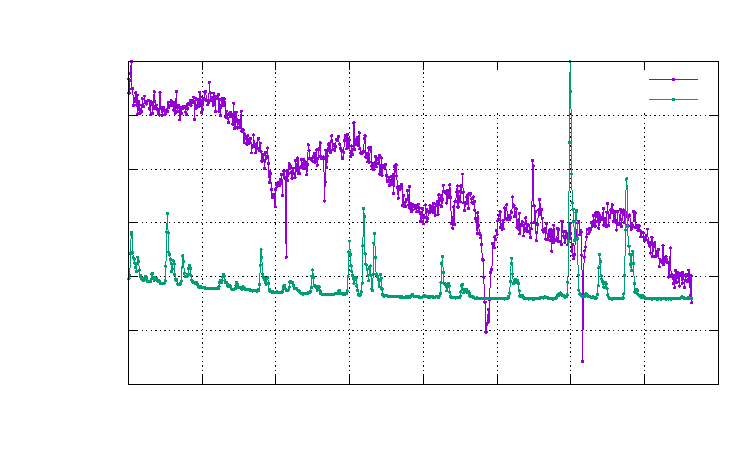
\includegraphics[width={360.00bp},height={216.00bp}]{21428-B3_data}}%
    \gplfronttext
  \end{picture}%
\endgroup
}
  \caption{}
\end{figure}
\begin{figure}[h]
  \centering
  \resizebox{.5\textwidth}{!}{% GNUPLOT: LaTeX picture with Postscript
\begingroup
  \makeatletter
  \providecommand\color[2][]{%
    \GenericError{(gnuplot) \space\space\space\@spaces}{%
      Package color not loaded in conjunction with
      terminal option `colourtext'%
    }{See the gnuplot documentation for explanation.%
    }{Either use 'blacktext' in gnuplot or load the package
      color.sty in LaTeX.}%
    \renewcommand\color[2][]{}%
  }%
  \providecommand\includegraphics[2][]{%
    \GenericError{(gnuplot) \space\space\space\@spaces}{%
      Package graphicx or graphics not loaded%
    }{See the gnuplot documentation for explanation.%
    }{The gnuplot epslatex terminal needs graphicx.sty or graphics.sty.}%
    \renewcommand\includegraphics[2][]{}%
  }%
  \providecommand\rotatebox[2]{#2}%
  \@ifundefined{ifGPcolor}{%
    \newif\ifGPcolor
    \GPcolortrue
  }{}%
  \@ifundefined{ifGPblacktext}{%
    \newif\ifGPblacktext
    \GPblacktexttrue
  }{}%
  % define a \g@addto@macro without @ in the name:
  \let\gplgaddtomacro\g@addto@macro
  % define empty templates for all commands taking text:
  \gdef\gplbacktext{}%
  \gdef\gplfronttext{}%
  \makeatother
  \ifGPblacktext
    % no textcolor at all
    \def\colorrgb#1{}%
    \def\colorgray#1{}%
  \else
    % gray or color?
    \ifGPcolor
      \def\colorrgb#1{\color[rgb]{#1}}%
      \def\colorgray#1{\color[gray]{#1}}%
      \expandafter\def\csname LTw\endcsname{\color{white}}%
      \expandafter\def\csname LTb\endcsname{\color{black}}%
      \expandafter\def\csname LTa\endcsname{\color{black}}%
      \expandafter\def\csname LT0\endcsname{\color[rgb]{1,0,0}}%
      \expandafter\def\csname LT1\endcsname{\color[rgb]{0,1,0}}%
      \expandafter\def\csname LT2\endcsname{\color[rgb]{0,0,1}}%
      \expandafter\def\csname LT3\endcsname{\color[rgb]{1,0,1}}%
      \expandafter\def\csname LT4\endcsname{\color[rgb]{0,1,1}}%
      \expandafter\def\csname LT5\endcsname{\color[rgb]{1,1,0}}%
      \expandafter\def\csname LT6\endcsname{\color[rgb]{0,0,0}}%
      \expandafter\def\csname LT7\endcsname{\color[rgb]{1,0.3,0}}%
      \expandafter\def\csname LT8\endcsname{\color[rgb]{0.5,0.5,0.5}}%
    \else
      % gray
      \def\colorrgb#1{\color{black}}%
      \def\colorgray#1{\color[gray]{#1}}%
      \expandafter\def\csname LTw\endcsname{\color{white}}%
      \expandafter\def\csname LTb\endcsname{\color{black}}%
      \expandafter\def\csname LTa\endcsname{\color{black}}%
      \expandafter\def\csname LT0\endcsname{\color{black}}%
      \expandafter\def\csname LT1\endcsname{\color{black}}%
      \expandafter\def\csname LT2\endcsname{\color{black}}%
      \expandafter\def\csname LT3\endcsname{\color{black}}%
      \expandafter\def\csname LT4\endcsname{\color{black}}%
      \expandafter\def\csname LT5\endcsname{\color{black}}%
      \expandafter\def\csname LT6\endcsname{\color{black}}%
      \expandafter\def\csname LT7\endcsname{\color{black}}%
      \expandafter\def\csname LT8\endcsname{\color{black}}%
    \fi
  \fi
    \setlength{\unitlength}{0.0500bp}%
    \ifx\gptboxheight\undefined%
      \newlength{\gptboxheight}%
      \newlength{\gptboxwidth}%
      \newsavebox{\gptboxtext}%
    \fi%
    \setlength{\fboxrule}{0.5pt}%
    \setlength{\fboxsep}{1pt}%
    \definecolor{tbcol}{rgb}{1,1,1}%
\begin{picture}(7200.00,4320.00)%
    \gplgaddtomacro\gplbacktext{%
      \csname LTb\endcsname%%
      \put(927,619){\makebox(0,0)[r]{\strut{}15\cdot10^{3}}}%
      \csname LTb\endcsname%%
      \put(927,901){\makebox(0,0)[r]{\strut{}16\cdot10^{3}}}%
      \csname LTb\endcsname%%
      \put(927,1182){\makebox(0,0)[r]{\strut{}17\cdot10^{3}}}%
      \csname LTb\endcsname%%
      \put(927,1464){\makebox(0,0)[r]{\strut{}18\cdot10^{3}}}%
      \csname LTb\endcsname%%
      \put(927,1746){\makebox(0,0)[r]{\strut{}19\cdot10^{3}}}%
      \csname LTb\endcsname%%
      \put(927,2028){\makebox(0,0)[r]{\strut{}20\cdot10^{3}}}%
      \csname LTb\endcsname%%
      \put(927,2310){\makebox(0,0)[r]{\strut{}21\cdot10^{3}}}%
      \csname LTb\endcsname%%
      \put(927,2592){\makebox(0,0)[r]{\strut{}22\cdot10^{3}}}%
      \csname LTb\endcsname%%
      \put(927,2873){\makebox(0,0)[r]{\strut{}23\cdot10^{3}}}%
      \csname LTb\endcsname%%
      \put(927,3155){\makebox(0,0)[r]{\strut{}24\cdot10^{3}}}%
      \csname LTb\endcsname%%
      \put(927,3437){\makebox(0,0)[r]{\strut{}25\cdot10^{3}}}%
      \csname LTb\endcsname%%
      \put(927,3719){\makebox(0,0)[r]{\strut{}26\cdot10^{3}}}%
      \csname LTb\endcsname%%
      \put(2197,425){\makebox(0,0){\strut{}650\cdot10^{-9}}}%
      \csname LTb\endcsname%%
      \put(3662,425){\makebox(0,0){\strut{}655\cdot10^{-9}}}%
      \csname LTb\endcsname%%
      \put(5128,425){\makebox(0,0){\strut{}660\cdot10^{-9}}}%
      \csname LTb\endcsname%%
      \put(6593,425){\makebox(0,0){\strut{}665\cdot10^{-9}}}%
    }%
    \gplgaddtomacro\gplfronttext{%
      \csname LTb\endcsname%%
      \put(6123,986){\makebox(0,0)[r]{\strut{}Datenpunkte}}%
      \csname LTb\endcsname%%
      \put(6123,793){\makebox(0,0)[r]{\strut{}Anpassung $G_\text{f}(x)$}}%
      \csname LTb\endcsname%%
      \put(170,2169){\rotatebox{-270.00}{\makebox(0,0){\strut{}Amplitude$/\textrm{a.u.}$}}}%
      \csname LTb\endcsname%%
      \put(3955,135){\makebox(0,0){\strut{}Wellenlänge $\lambda/\SI{}{m}$}}%
      \csname LTb\endcsname%%
      \put(3955,4009){\makebox(0,0){\strut{}H$\alpha$(\SI{656}{nm})-Linie von 21428-B3 mit $\chi^2/\textrm{ddof}=\SI{4.66E-01}{}$}}%
    }%
    \gplbacktext
    \put(0,0){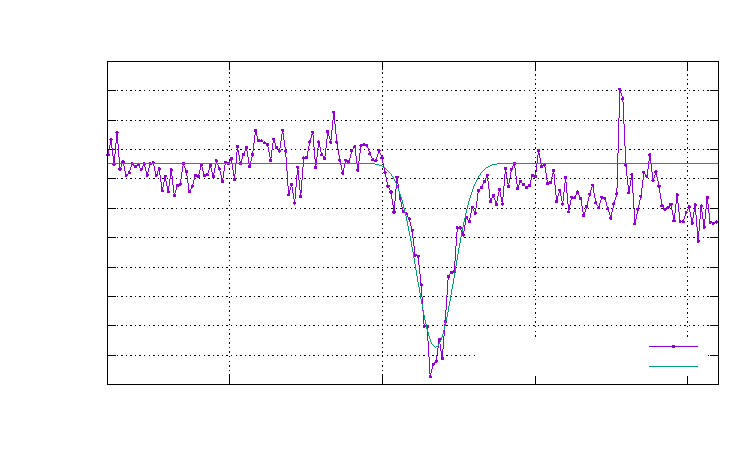
\includegraphics[width={360.00bp},height={216.00bp}]{21428-B3_gauss}}%
    \gplfronttext
  \end{picture}%
\endgroup
}
  \caption{}
\end{figure}
\begin{figure}[h]
  \centering
  \resizebox{.5\textwidth}{!}{% GNUPLOT: LaTeX picture with Postscript
\begingroup
  \makeatletter
  \providecommand\color[2][]{%
    \GenericError{(gnuplot) \space\space\space\@spaces}{%
      Package color not loaded in conjunction with
      terminal option `colourtext'%
    }{See the gnuplot documentation for explanation.%
    }{Either use 'blacktext' in gnuplot or load the package
      color.sty in LaTeX.}%
    \renewcommand\color[2][]{}%
  }%
  \providecommand\includegraphics[2][]{%
    \GenericError{(gnuplot) \space\space\space\@spaces}{%
      Package graphicx or graphics not loaded%
    }{See the gnuplot documentation for explanation.%
    }{The gnuplot epslatex terminal needs graphicx.sty or graphics.sty.}%
    \renewcommand\includegraphics[2][]{}%
  }%
  \providecommand\rotatebox[2]{#2}%
  \@ifundefined{ifGPcolor}{%
    \newif\ifGPcolor
    \GPcolortrue
  }{}%
  \@ifundefined{ifGPblacktext}{%
    \newif\ifGPblacktext
    \GPblacktexttrue
  }{}%
  % define a \g@addto@macro without @ in the name:
  \let\gplgaddtomacro\g@addto@macro
  % define empty templates for all commands taking text:
  \gdef\gplbacktext{}%
  \gdef\gplfronttext{}%
  \makeatother
  \ifGPblacktext
    % no textcolor at all
    \def\colorrgb#1{}%
    \def\colorgray#1{}%
  \else
    % gray or color?
    \ifGPcolor
      \def\colorrgb#1{\color[rgb]{#1}}%
      \def\colorgray#1{\color[gray]{#1}}%
      \expandafter\def\csname LTw\endcsname{\color{white}}%
      \expandafter\def\csname LTb\endcsname{\color{black}}%
      \expandafter\def\csname LTa\endcsname{\color{black}}%
      \expandafter\def\csname LT0\endcsname{\color[rgb]{1,0,0}}%
      \expandafter\def\csname LT1\endcsname{\color[rgb]{0,1,0}}%
      \expandafter\def\csname LT2\endcsname{\color[rgb]{0,0,1}}%
      \expandafter\def\csname LT3\endcsname{\color[rgb]{1,0,1}}%
      \expandafter\def\csname LT4\endcsname{\color[rgb]{0,1,1}}%
      \expandafter\def\csname LT5\endcsname{\color[rgb]{1,1,0}}%
      \expandafter\def\csname LT6\endcsname{\color[rgb]{0,0,0}}%
      \expandafter\def\csname LT7\endcsname{\color[rgb]{1,0.3,0}}%
      \expandafter\def\csname LT8\endcsname{\color[rgb]{0.5,0.5,0.5}}%
    \else
      % gray
      \def\colorrgb#1{\color{black}}%
      \def\colorgray#1{\color[gray]{#1}}%
      \expandafter\def\csname LTw\endcsname{\color{white}}%
      \expandafter\def\csname LTb\endcsname{\color{black}}%
      \expandafter\def\csname LTa\endcsname{\color{black}}%
      \expandafter\def\csname LT0\endcsname{\color{black}}%
      \expandafter\def\csname LT1\endcsname{\color{black}}%
      \expandafter\def\csname LT2\endcsname{\color{black}}%
      \expandafter\def\csname LT3\endcsname{\color{black}}%
      \expandafter\def\csname LT4\endcsname{\color{black}}%
      \expandafter\def\csname LT5\endcsname{\color{black}}%
      \expandafter\def\csname LT6\endcsname{\color{black}}%
      \expandafter\def\csname LT7\endcsname{\color{black}}%
      \expandafter\def\csname LT8\endcsname{\color{black}}%
    \fi
  \fi
    \setlength{\unitlength}{0.0500bp}%
    \ifx\gptboxheight\undefined%
      \newlength{\gptboxheight}%
      \newlength{\gptboxwidth}%
      \newsavebox{\gptboxtext}%
    \fi%
    \setlength{\fboxrule}{0.5pt}%
    \setlength{\fboxsep}{1pt}%
    \definecolor{tbcol}{rgb}{1,1,1}%
\begin{picture}(7200.00,4320.00)%
    \gplgaddtomacro\gplbacktext{%
      \csname LTb\endcsname%%
      \put(1123,619){\makebox(0,0)[r]{\strut{}$635\cdot10^{-9}$}}%
      \csname LTb\endcsname%%
      \put(1123,963){\makebox(0,0)[r]{\strut{}$640\cdot10^{-9}$}}%
      \csname LTb\endcsname%%
      \put(1123,1308){\makebox(0,0)[r]{\strut{}$645\cdot10^{-9}$}}%
      \csname LTb\endcsname%%
      \put(1123,1652){\makebox(0,0)[r]{\strut{}$650\cdot10^{-9}$}}%
      \csname LTb\endcsname%%
      \put(1123,1997){\makebox(0,0)[r]{\strut{}$655\cdot10^{-9}$}}%
      \csname LTb\endcsname%%
      \put(1123,2341){\makebox(0,0)[r]{\strut{}$660\cdot10^{-9}$}}%
      \csname LTb\endcsname%%
      \put(1123,2686){\makebox(0,0)[r]{\strut{}$665\cdot10^{-9}$}}%
      \csname LTb\endcsname%%
      \put(1123,3030){\makebox(0,0)[r]{\strut{}$670\cdot10^{-9}$}}%
      \csname LTb\endcsname%%
      \put(1123,3374){\makebox(0,0)[r]{\strut{}$675\cdot10^{-9}$}}%
      \csname LTb\endcsname%%
      \put(1123,3719){\makebox(0,0)[r]{\strut{}$680\cdot10^{-9}$}}%
      \csname LTb\endcsname%%
      \put(1221,425){\makebox(0,0){\strut{}$300$}}%
      \csname LTb\endcsname%%
      \put(1929,425){\makebox(0,0){\strut{}$350$}}%
      \csname LTb\endcsname%%
      \put(2637,425){\makebox(0,0){\strut{}$400$}}%
      \csname LTb\endcsname%%
      \put(3345,425){\makebox(0,0){\strut{}$450$}}%
      \csname LTb\endcsname%%
      \put(4053,425){\makebox(0,0){\strut{}$500$}}%
      \csname LTb\endcsname%%
      \put(4761,425){\makebox(0,0){\strut{}$550$}}%
      \csname LTb\endcsname%%
      \put(5470,425){\makebox(0,0){\strut{}$600$}}%
      \csname LTb\endcsname%%
      \put(6178,425){\makebox(0,0){\strut{}$650$}}%
      \csname LTb\endcsname%%
      \put(6886,425){\makebox(0,0){\strut{}$700$}}%
    }%
    \gplgaddtomacro\gplfronttext{%
      \csname LTb\endcsname%%
      \put(170,2169){\rotatebox{-270}{\makebox(0,0){\strut{}Wellenlänge $\lambda/\SI{}{m}$}}}%
      \csname LTb\endcsname%%
      \put(4053,135){\makebox(0,0){\strut{}Pixelkoordinate$/\textrm{Pixel}$}}%
      \csname LTb\endcsname%%
      \put(6123,3545){\makebox(0,0)[r]{\strut{}Datenpunkte}}%
      \csname LTb\endcsname%%
      \put(6123,3351){\makebox(0,0)[r]{\strut{}Anpassung $\lambda_\text{f}(x)$}}%
      \csname LTb\endcsname%%
      \put(4053,4009){\makebox(0,0){\strut{}Kalibraiton des 21428-B3 Spektrums mit $\chi^2/\textrm{ddof}=\SI{3.03E-02}{}$}}%
    }%
    \gplbacktext
    \put(0,0){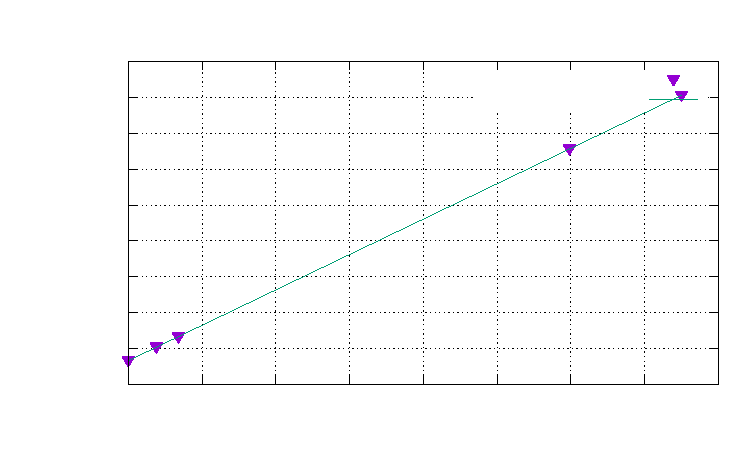
\includegraphics[width={360.00bp},height={216.00bp}]{21428-B3_kali}}%
    \gplfronttext
  \end{picture}%
\endgroup
}
  \caption{}
\end{figure}
\begin{figure}[h]
  \centering
  \resizebox{.5\textwidth}{!}{% GNUPLOT: LaTeX picture with Postscript
\begingroup
  \makeatletter
  \providecommand\color[2][]{%
    \GenericError{(gnuplot) \space\space\space\@spaces}{%
      Package color not loaded in conjunction with
      terminal option `colourtext'%
    }{See the gnuplot documentation for explanation.%
    }{Either use 'blacktext' in gnuplot or load the package
      color.sty in LaTeX.}%
    \renewcommand\color[2][]{}%
  }%
  \providecommand\includegraphics[2][]{%
    \GenericError{(gnuplot) \space\space\space\@spaces}{%
      Package graphicx or graphics not loaded%
    }{See the gnuplot documentation for explanation.%
    }{The gnuplot epslatex terminal needs graphicx.sty or graphics.sty.}%
    \renewcommand\includegraphics[2][]{}%
  }%
  \providecommand\rotatebox[2]{#2}%
  \@ifundefined{ifGPcolor}{%
    \newif\ifGPcolor
    \GPcolortrue
  }{}%
  \@ifundefined{ifGPblacktext}{%
    \newif\ifGPblacktext
    \GPblacktexttrue
  }{}%
  % define a \g@addto@macro without @ in the name:
  \let\gplgaddtomacro\g@addto@macro
  % define empty templates for all commands taking text:
  \gdef\gplbacktext{}%
  \gdef\gplfronttext{}%
  \makeatother
  \ifGPblacktext
    % no textcolor at all
    \def\colorrgb#1{}%
    \def\colorgray#1{}%
  \else
    % gray or color?
    \ifGPcolor
      \def\colorrgb#1{\color[rgb]{#1}}%
      \def\colorgray#1{\color[gray]{#1}}%
      \expandafter\def\csname LTw\endcsname{\color{white}}%
      \expandafter\def\csname LTb\endcsname{\color{black}}%
      \expandafter\def\csname LTa\endcsname{\color{black}}%
      \expandafter\def\csname LT0\endcsname{\color[rgb]{1,0,0}}%
      \expandafter\def\csname LT1\endcsname{\color[rgb]{0,1,0}}%
      \expandafter\def\csname LT2\endcsname{\color[rgb]{0,0,1}}%
      \expandafter\def\csname LT3\endcsname{\color[rgb]{1,0,1}}%
      \expandafter\def\csname LT4\endcsname{\color[rgb]{0,1,1}}%
      \expandafter\def\csname LT5\endcsname{\color[rgb]{1,1,0}}%
      \expandafter\def\csname LT6\endcsname{\color[rgb]{0,0,0}}%
      \expandafter\def\csname LT7\endcsname{\color[rgb]{1,0.3,0}}%
      \expandafter\def\csname LT8\endcsname{\color[rgb]{0.5,0.5,0.5}}%
    \else
      % gray
      \def\colorrgb#1{\color{black}}%
      \def\colorgray#1{\color[gray]{#1}}%
      \expandafter\def\csname LTw\endcsname{\color{white}}%
      \expandafter\def\csname LTb\endcsname{\color{black}}%
      \expandafter\def\csname LTa\endcsname{\color{black}}%
      \expandafter\def\csname LT0\endcsname{\color{black}}%
      \expandafter\def\csname LT1\endcsname{\color{black}}%
      \expandafter\def\csname LT2\endcsname{\color{black}}%
      \expandafter\def\csname LT3\endcsname{\color{black}}%
      \expandafter\def\csname LT4\endcsname{\color{black}}%
      \expandafter\def\csname LT5\endcsname{\color{black}}%
      \expandafter\def\csname LT6\endcsname{\color{black}}%
      \expandafter\def\csname LT7\endcsname{\color{black}}%
      \expandafter\def\csname LT8\endcsname{\color{black}}%
    \fi
  \fi
    \setlength{\unitlength}{0.0500bp}%
    \ifx\gptboxheight\undefined%
      \newlength{\gptboxheight}%
      \newlength{\gptboxwidth}%
      \newsavebox{\gptboxtext}%
    \fi%
    \setlength{\fboxrule}{0.5pt}%
    \setlength{\fboxsep}{1pt}%
    \definecolor{tbcol}{rgb}{1,1,1}%
\begin{picture}(7200.00,4320.00)%
    \gplgaddtomacro\gplbacktext{%
      \csname LTb\endcsname%%
      \put(1123,619){\makebox(0,0)[r]{\strut{}$300\cdot10^{-3}$}}%
      \csname LTb\endcsname%%
      \put(1123,1062){\makebox(0,0)[r]{\strut{}$400\cdot10^{-3}$}}%
      \csname LTb\endcsname%%
      \put(1123,1505){\makebox(0,0)[r]{\strut{}$500\cdot10^{-3}$}}%
      \csname LTb\endcsname%%
      \put(1123,1947){\makebox(0,0)[r]{\strut{}$600\cdot10^{-3}$}}%
      \csname LTb\endcsname%%
      \put(1123,2390){\makebox(0,0)[r]{\strut{}$700\cdot10^{-3}$}}%
      \csname LTb\endcsname%%
      \put(1123,2833){\makebox(0,0)[r]{\strut{}$800\cdot10^{-3}$}}%
      \csname LTb\endcsname%%
      \put(1123,3276){\makebox(0,0)[r]{\strut{}$900\cdot10^{-3}$}}%
      \csname LTb\endcsname%%
      \put(1123,3719){\makebox(0,0)[r]{\strut{}$1\cdot10^{0}$}}%
      \csname LTb\endcsname%%
      \put(1221,425){\makebox(0,0){\strut{}$0$}}%
      \csname LTb\endcsname%%
      \put(1929,425){\makebox(0,0){\strut{}$100$}}%
      \csname LTb\endcsname%%
      \put(2637,425){\makebox(0,0){\strut{}$200$}}%
      \csname LTb\endcsname%%
      \put(3345,425){\makebox(0,0){\strut{}$300$}}%
      \csname LTb\endcsname%%
      \put(4053,425){\makebox(0,0){\strut{}$400$}}%
      \csname LTb\endcsname%%
      \put(4761,425){\makebox(0,0){\strut{}$500$}}%
      \csname LTb\endcsname%%
      \put(5470,425){\makebox(0,0){\strut{}$600$}}%
      \csname LTb\endcsname%%
      \put(6178,425){\makebox(0,0){\strut{}$700$}}%
      \csname LTb\endcsname%%
      \put(6886,425){\makebox(0,0){\strut{}$800$}}%
    }%
    \gplgaddtomacro\gplfronttext{%
      \csname LTb\endcsname%%
      \put(170,2169){\rotatebox{-270}{\makebox(0,0){\strut{}Amplitude$/\textrm{a.u.}$}}}%
      \csname LTb\endcsname%%
      \put(4053,135){\makebox(0,0){\strut{}Pixelkoordinate$/\textrm{Pixel}$}}%
      \csname LTb\endcsname%%
      \put(6123,3545){\makebox(0,0)[r]{\strut{}29488-A5}}%
      \csname LTb\endcsname%%
      \put(6123,3351){\makebox(0,0)[r]{\strut{}Kalibrationslampe}}%
      \csname LTb\endcsname%%
      \put(4053,4009){\makebox(0,0){\strut{}Spektrum}}%
    }%
    \gplbacktext
    \put(0,0){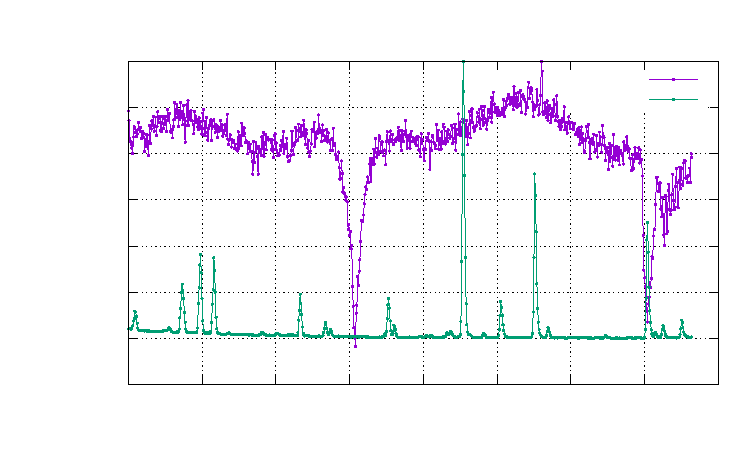
\includegraphics[width={360.00bp},height={216.00bp}]{29488-A5_data}}%
    \gplfronttext
  \end{picture}%
\endgroup
}
  \caption{}
\end{figure}
\begin{figure}[h]
  \centering
  \resizebox{.5\textwidth}{!}{% GNUPLOT: LaTeX picture with Postscript
\begingroup
  \makeatletter
  \providecommand\color[2][]{%
    \GenericError{(gnuplot) \space\space\space\@spaces}{%
      Package color not loaded in conjunction with
      terminal option `colourtext'%
    }{See the gnuplot documentation for explanation.%
    }{Either use 'blacktext' in gnuplot or load the package
      color.sty in LaTeX.}%
    \renewcommand\color[2][]{}%
  }%
  \providecommand\includegraphics[2][]{%
    \GenericError{(gnuplot) \space\space\space\@spaces}{%
      Package graphicx or graphics not loaded%
    }{See the gnuplot documentation for explanation.%
    }{The gnuplot epslatex terminal needs graphicx.sty or graphics.sty.}%
    \renewcommand\includegraphics[2][]{}%
  }%
  \providecommand\rotatebox[2]{#2}%
  \@ifundefined{ifGPcolor}{%
    \newif\ifGPcolor
    \GPcolortrue
  }{}%
  \@ifundefined{ifGPblacktext}{%
    \newif\ifGPblacktext
    \GPblacktexttrue
  }{}%
  % define a \g@addto@macro without @ in the name:
  \let\gplgaddtomacro\g@addto@macro
  % define empty templates for all commands taking text:
  \gdef\gplbacktext{}%
  \gdef\gplfronttext{}%
  \makeatother
  \ifGPblacktext
    % no textcolor at all
    \def\colorrgb#1{}%
    \def\colorgray#1{}%
  \else
    % gray or color?
    \ifGPcolor
      \def\colorrgb#1{\color[rgb]{#1}}%
      \def\colorgray#1{\color[gray]{#1}}%
      \expandafter\def\csname LTw\endcsname{\color{white}}%
      \expandafter\def\csname LTb\endcsname{\color{black}}%
      \expandafter\def\csname LTa\endcsname{\color{black}}%
      \expandafter\def\csname LT0\endcsname{\color[rgb]{1,0,0}}%
      \expandafter\def\csname LT1\endcsname{\color[rgb]{0,1,0}}%
      \expandafter\def\csname LT2\endcsname{\color[rgb]{0,0,1}}%
      \expandafter\def\csname LT3\endcsname{\color[rgb]{1,0,1}}%
      \expandafter\def\csname LT4\endcsname{\color[rgb]{0,1,1}}%
      \expandafter\def\csname LT5\endcsname{\color[rgb]{1,1,0}}%
      \expandafter\def\csname LT6\endcsname{\color[rgb]{0,0,0}}%
      \expandafter\def\csname LT7\endcsname{\color[rgb]{1,0.3,0}}%
      \expandafter\def\csname LT8\endcsname{\color[rgb]{0.5,0.5,0.5}}%
    \else
      % gray
      \def\colorrgb#1{\color{black}}%
      \def\colorgray#1{\color[gray]{#1}}%
      \expandafter\def\csname LTw\endcsname{\color{white}}%
      \expandafter\def\csname LTb\endcsname{\color{black}}%
      \expandafter\def\csname LTa\endcsname{\color{black}}%
      \expandafter\def\csname LT0\endcsname{\color{black}}%
      \expandafter\def\csname LT1\endcsname{\color{black}}%
      \expandafter\def\csname LT2\endcsname{\color{black}}%
      \expandafter\def\csname LT3\endcsname{\color{black}}%
      \expandafter\def\csname LT4\endcsname{\color{black}}%
      \expandafter\def\csname LT5\endcsname{\color{black}}%
      \expandafter\def\csname LT6\endcsname{\color{black}}%
      \expandafter\def\csname LT7\endcsname{\color{black}}%
      \expandafter\def\csname LT8\endcsname{\color{black}}%
    \fi
  \fi
    \setlength{\unitlength}{0.0500bp}%
    \ifx\gptboxheight\undefined%
      \newlength{\gptboxheight}%
      \newlength{\gptboxwidth}%
      \newsavebox{\gptboxtext}%
    \fi%
    \setlength{\fboxrule}{0.5pt}%
    \setlength{\fboxsep}{1pt}%
    \definecolor{tbcol}{rgb}{1,1,1}%
\begin{picture}(7200.00,4320.00)%
    \gplgaddtomacro\gplbacktext{%
      \csname LTb\endcsname%%
      \put(927,619){\makebox(0,0)[r]{\strut{}8\cdot10^{3}}}%
      \csname LTb\endcsname%%
      \put(927,1062){\makebox(0,0)[r]{\strut{}10\cdot10^{3}}}%
      \csname LTb\endcsname%%
      \put(927,1505){\makebox(0,0)[r]{\strut{}12\cdot10^{3}}}%
      \csname LTb\endcsname%%
      \put(927,1947){\makebox(0,0)[r]{\strut{}14\cdot10^{3}}}%
      \csname LTb\endcsname%%
      \put(927,2390){\makebox(0,0)[r]{\strut{}16\cdot10^{3}}}%
      \csname LTb\endcsname%%
      \put(927,2833){\makebox(0,0)[r]{\strut{}18\cdot10^{3}}}%
      \csname LTb\endcsname%%
      \put(927,3276){\makebox(0,0)[r]{\strut{}20\cdot10^{3}}}%
      \csname LTb\endcsname%%
      \put(927,3719){\makebox(0,0)[r]{\strut{}22\cdot10^{3}}}%
      \csname LTb\endcsname%%
      \put(2197,425){\makebox(0,0){\strut{}650\cdot10^{-9}}}%
      \csname LTb\endcsname%%
      \put(3662,425){\makebox(0,0){\strut{}655\cdot10^{-9}}}%
      \csname LTb\endcsname%%
      \put(5128,425){\makebox(0,0){\strut{}660\cdot10^{-9}}}%
      \csname LTb\endcsname%%
      \put(6593,425){\makebox(0,0){\strut{}665\cdot10^{-9}}}%
    }%
    \gplgaddtomacro\gplfronttext{%
      \csname LTb\endcsname%%
      \put(6123,986){\makebox(0,0)[r]{\strut{}Datenpunkte}}%
      \csname LTb\endcsname%%
      \put(6123,793){\makebox(0,0)[r]{\strut{}Anpassung $G_\text{f}(x)$}}%
      \csname LTb\endcsname%%
      \put(170,2169){\rotatebox{-270.00}{\makebox(0,0){\strut{}Amplitude$/\textrm{a.u.}$}}}%
      \csname LTb\endcsname%%
      \put(3955,135){\makebox(0,0){\strut{}Wellenlänge $\lambda/\SI{}{m}$}}%
      \csname LTb\endcsname%%
      \put(3955,4009){\makebox(0,0){\strut{}H$\alpha$(\SI{656}{nm})-Linie von 29488-A5 mit $\chi^2/\textrm{ddof}=\SI{4.43E-01}{}$}}%
    }%
    \gplbacktext
    \put(0,0){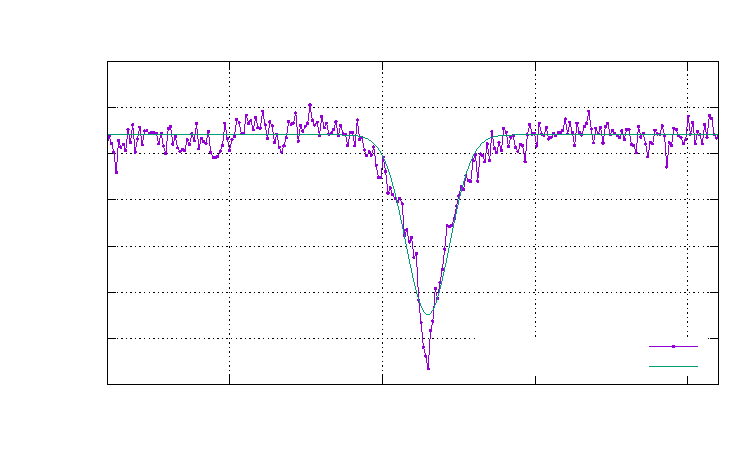
\includegraphics[width={360.00bp},height={216.00bp}]{29488-A5_gauss}}%
    \gplfronttext
  \end{picture}%
\endgroup
}
  \caption{}
\end{figure}
\begin{figure}[h]
  \centering
  \resizebox{.5\textwidth}{!}{% GNUPLOT: LaTeX picture with Postscript
\begingroup
  \makeatletter
  \providecommand\color[2][]{%
    \GenericError{(gnuplot) \space\space\space\@spaces}{%
      Package color not loaded in conjunction with
      terminal option `colourtext'%
    }{See the gnuplot documentation for explanation.%
    }{Either use 'blacktext' in gnuplot or load the package
      color.sty in LaTeX.}%
    \renewcommand\color[2][]{}%
  }%
  \providecommand\includegraphics[2][]{%
    \GenericError{(gnuplot) \space\space\space\@spaces}{%
      Package graphicx or graphics not loaded%
    }{See the gnuplot documentation for explanation.%
    }{The gnuplot epslatex terminal needs graphicx.sty or graphics.sty.}%
    \renewcommand\includegraphics[2][]{}%
  }%
  \providecommand\rotatebox[2]{#2}%
  \@ifundefined{ifGPcolor}{%
    \newif\ifGPcolor
    \GPcolortrue
  }{}%
  \@ifundefined{ifGPblacktext}{%
    \newif\ifGPblacktext
    \GPblacktexttrue
  }{}%
  % define a \g@addto@macro without @ in the name:
  \let\gplgaddtomacro\g@addto@macro
  % define empty templates for all commands taking text:
  \gdef\gplbacktext{}%
  \gdef\gplfronttext{}%
  \makeatother
  \ifGPblacktext
    % no textcolor at all
    \def\colorrgb#1{}%
    \def\colorgray#1{}%
  \else
    % gray or color?
    \ifGPcolor
      \def\colorrgb#1{\color[rgb]{#1}}%
      \def\colorgray#1{\color[gray]{#1}}%
      \expandafter\def\csname LTw\endcsname{\color{white}}%
      \expandafter\def\csname LTb\endcsname{\color{black}}%
      \expandafter\def\csname LTa\endcsname{\color{black}}%
      \expandafter\def\csname LT0\endcsname{\color[rgb]{1,0,0}}%
      \expandafter\def\csname LT1\endcsname{\color[rgb]{0,1,0}}%
      \expandafter\def\csname LT2\endcsname{\color[rgb]{0,0,1}}%
      \expandafter\def\csname LT3\endcsname{\color[rgb]{1,0,1}}%
      \expandafter\def\csname LT4\endcsname{\color[rgb]{0,1,1}}%
      \expandafter\def\csname LT5\endcsname{\color[rgb]{1,1,0}}%
      \expandafter\def\csname LT6\endcsname{\color[rgb]{0,0,0}}%
      \expandafter\def\csname LT7\endcsname{\color[rgb]{1,0.3,0}}%
      \expandafter\def\csname LT8\endcsname{\color[rgb]{0.5,0.5,0.5}}%
    \else
      % gray
      \def\colorrgb#1{\color{black}}%
      \def\colorgray#1{\color[gray]{#1}}%
      \expandafter\def\csname LTw\endcsname{\color{white}}%
      \expandafter\def\csname LTb\endcsname{\color{black}}%
      \expandafter\def\csname LTa\endcsname{\color{black}}%
      \expandafter\def\csname LT0\endcsname{\color{black}}%
      \expandafter\def\csname LT1\endcsname{\color{black}}%
      \expandafter\def\csname LT2\endcsname{\color{black}}%
      \expandafter\def\csname LT3\endcsname{\color{black}}%
      \expandafter\def\csname LT4\endcsname{\color{black}}%
      \expandafter\def\csname LT5\endcsname{\color{black}}%
      \expandafter\def\csname LT6\endcsname{\color{black}}%
      \expandafter\def\csname LT7\endcsname{\color{black}}%
      \expandafter\def\csname LT8\endcsname{\color{black}}%
    \fi
  \fi
    \setlength{\unitlength}{0.0500bp}%
    \ifx\gptboxheight\undefined%
      \newlength{\gptboxheight}%
      \newlength{\gptboxwidth}%
      \newsavebox{\gptboxtext}%
    \fi%
    \setlength{\fboxrule}{0.5pt}%
    \setlength{\fboxsep}{1pt}%
    \definecolor{tbcol}{rgb}{1,1,1}%
\begin{picture}(7200.00,4320.00)%
    \gplgaddtomacro\gplbacktext{%
      \csname LTb\endcsname%%
      \put(1123,619){\makebox(0,0)[r]{\strut{}$635\cdot10^{-9}$}}%
      \csname LTb\endcsname%%
      \put(1123,963){\makebox(0,0)[r]{\strut{}$640\cdot10^{-9}$}}%
      \csname LTb\endcsname%%
      \put(1123,1308){\makebox(0,0)[r]{\strut{}$645\cdot10^{-9}$}}%
      \csname LTb\endcsname%%
      \put(1123,1652){\makebox(0,0)[r]{\strut{}$650\cdot10^{-9}$}}%
      \csname LTb\endcsname%%
      \put(1123,1997){\makebox(0,0)[r]{\strut{}$655\cdot10^{-9}$}}%
      \csname LTb\endcsname%%
      \put(1123,2341){\makebox(0,0)[r]{\strut{}$660\cdot10^{-9}$}}%
      \csname LTb\endcsname%%
      \put(1123,2686){\makebox(0,0)[r]{\strut{}$665\cdot10^{-9}$}}%
      \csname LTb\endcsname%%
      \put(1123,3030){\makebox(0,0)[r]{\strut{}$670\cdot10^{-9}$}}%
      \csname LTb\endcsname%%
      \put(1123,3374){\makebox(0,0)[r]{\strut{}$675\cdot10^{-9}$}}%
      \csname LTb\endcsname%%
      \put(1123,3719){\makebox(0,0)[r]{\strut{}$680\cdot10^{-9}$}}%
      \csname LTb\endcsname%%
      \put(1221,425){\makebox(0,0){\strut{}$50$}}%
      \csname LTb\endcsname%%
      \put(1736,425){\makebox(0,0){\strut{}$100$}}%
      \csname LTb\endcsname%%
      \put(2251,425){\makebox(0,0){\strut{}$150$}}%
      \csname LTb\endcsname%%
      \put(2766,425){\makebox(0,0){\strut{}$200$}}%
      \csname LTb\endcsname%%
      \put(3281,425){\makebox(0,0){\strut{}$250$}}%
      \csname LTb\endcsname%%
      \put(3796,425){\makebox(0,0){\strut{}$300$}}%
      \csname LTb\endcsname%%
      \put(4311,425){\makebox(0,0){\strut{}$350$}}%
      \csname LTb\endcsname%%
      \put(4826,425){\makebox(0,0){\strut{}$400$}}%
      \csname LTb\endcsname%%
      \put(5341,425){\makebox(0,0){\strut{}$450$}}%
      \csname LTb\endcsname%%
      \put(5856,425){\makebox(0,0){\strut{}$500$}}%
      \csname LTb\endcsname%%
      \put(6371,425){\makebox(0,0){\strut{}$550$}}%
      \csname LTb\endcsname%%
      \put(6886,425){\makebox(0,0){\strut{}$600$}}%
    }%
    \gplgaddtomacro\gplfronttext{%
      \csname LTb\endcsname%%
      \put(170,2169){\rotatebox{-270}{\makebox(0,0){\strut{}Wellenlänge $\lambda/\SI{}{m}$}}}%
      \csname LTb\endcsname%%
      \put(4053,135){\makebox(0,0){\strut{}Pixelkoordinate$/\textrm{Pixel}$}}%
      \csname LTb\endcsname%%
      \put(6123,3545){\makebox(0,0)[r]{\strut{}Datenpunkte}}%
      \csname LTb\endcsname%%
      \put(6123,3351){\makebox(0,0)[r]{\strut{}Anpassung $\lambda_\text{f}(x)$}}%
      \csname LTb\endcsname%%
      \put(4053,4009){\makebox(0,0){\strut{}Kalibraiton des 29488-A5 Spektrums mit $\chi^2/\textrm{ddof}=\SI{1.69E-02}{}$}}%
    }%
    \gplbacktext
    \put(0,0){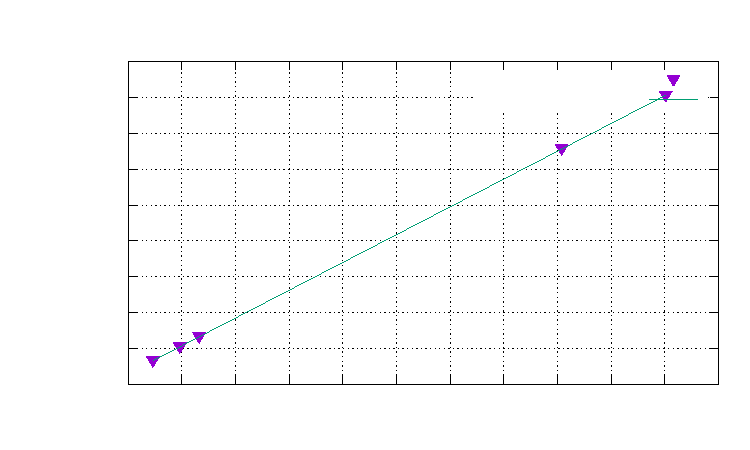
\includegraphics[width={360.00bp},height={216.00bp}]{29488-A5_kali}}%
    \gplfronttext
  \end{picture}%
\endgroup
}
  \caption{}
\end{figure}
\begin{figure}[h]
  \centering
  \resizebox{.5\textwidth}{!}{% GNUPLOT: LaTeX picture with Postscript
\begingroup
  \makeatletter
  \providecommand\color[2][]{%
    \GenericError{(gnuplot) \space\space\space\@spaces}{%
      Package color not loaded in conjunction with
      terminal option `colourtext'%
    }{See the gnuplot documentation for explanation.%
    }{Either use 'blacktext' in gnuplot or load the package
      color.sty in LaTeX.}%
    \renewcommand\color[2][]{}%
  }%
  \providecommand\includegraphics[2][]{%
    \GenericError{(gnuplot) \space\space\space\@spaces}{%
      Package graphicx or graphics not loaded%
    }{See the gnuplot documentation for explanation.%
    }{The gnuplot epslatex terminal needs graphicx.sty or graphics.sty.}%
    \renewcommand\includegraphics[2][]{}%
  }%
  \providecommand\rotatebox[2]{#2}%
  \@ifundefined{ifGPcolor}{%
    \newif\ifGPcolor
    \GPcolortrue
  }{}%
  \@ifundefined{ifGPblacktext}{%
    \newif\ifGPblacktext
    \GPblacktexttrue
  }{}%
  % define a \g@addto@macro without @ in the name:
  \let\gplgaddtomacro\g@addto@macro
  % define empty templates for all commands taking text:
  \gdef\gplbacktext{}%
  \gdef\gplfronttext{}%
  \makeatother
  \ifGPblacktext
    % no textcolor at all
    \def\colorrgb#1{}%
    \def\colorgray#1{}%
  \else
    % gray or color?
    \ifGPcolor
      \def\colorrgb#1{\color[rgb]{#1}}%
      \def\colorgray#1{\color[gray]{#1}}%
      \expandafter\def\csname LTw\endcsname{\color{white}}%
      \expandafter\def\csname LTb\endcsname{\color{black}}%
      \expandafter\def\csname LTa\endcsname{\color{black}}%
      \expandafter\def\csname LT0\endcsname{\color[rgb]{1,0,0}}%
      \expandafter\def\csname LT1\endcsname{\color[rgb]{0,1,0}}%
      \expandafter\def\csname LT2\endcsname{\color[rgb]{0,0,1}}%
      \expandafter\def\csname LT3\endcsname{\color[rgb]{1,0,1}}%
      \expandafter\def\csname LT4\endcsname{\color[rgb]{0,1,1}}%
      \expandafter\def\csname LT5\endcsname{\color[rgb]{1,1,0}}%
      \expandafter\def\csname LT6\endcsname{\color[rgb]{0,0,0}}%
      \expandafter\def\csname LT7\endcsname{\color[rgb]{1,0.3,0}}%
      \expandafter\def\csname LT8\endcsname{\color[rgb]{0.5,0.5,0.5}}%
    \else
      % gray
      \def\colorrgb#1{\color{black}}%
      \def\colorgray#1{\color[gray]{#1}}%
      \expandafter\def\csname LTw\endcsname{\color{white}}%
      \expandafter\def\csname LTb\endcsname{\color{black}}%
      \expandafter\def\csname LTa\endcsname{\color{black}}%
      \expandafter\def\csname LT0\endcsname{\color{black}}%
      \expandafter\def\csname LT1\endcsname{\color{black}}%
      \expandafter\def\csname LT2\endcsname{\color{black}}%
      \expandafter\def\csname LT3\endcsname{\color{black}}%
      \expandafter\def\csname LT4\endcsname{\color{black}}%
      \expandafter\def\csname LT5\endcsname{\color{black}}%
      \expandafter\def\csname LT6\endcsname{\color{black}}%
      \expandafter\def\csname LT7\endcsname{\color{black}}%
      \expandafter\def\csname LT8\endcsname{\color{black}}%
    \fi
  \fi
    \setlength{\unitlength}{0.0500bp}%
    \ifx\gptboxheight\undefined%
      \newlength{\gptboxheight}%
      \newlength{\gptboxwidth}%
      \newsavebox{\gptboxtext}%
    \fi%
    \setlength{\fboxrule}{0.5pt}%
    \setlength{\fboxsep}{1pt}%
    \definecolor{tbcol}{rgb}{1,1,1}%
\begin{picture}(7200.00,4320.00)%
    \gplgaddtomacro\gplbacktext{%
      \csname LTb\endcsname%%
      \put(1123,619){\makebox(0,0)[r]{\strut{}300\cdot10^{-3}}}%
      \csname LTb\endcsname%%
      \put(1123,1062){\makebox(0,0)[r]{\strut{}400\cdot10^{-3}}}%
      \csname LTb\endcsname%%
      \put(1123,1505){\makebox(0,0)[r]{\strut{}500\cdot10^{-3}}}%
      \csname LTb\endcsname%%
      \put(1123,1947){\makebox(0,0)[r]{\strut{}600\cdot10^{-3}}}%
      \csname LTb\endcsname%%
      \put(1123,2390){\makebox(0,0)[r]{\strut{}700\cdot10^{-3}}}%
      \csname LTb\endcsname%%
      \put(1123,2833){\makebox(0,0)[r]{\strut{}800\cdot10^{-3}}}%
      \csname LTb\endcsname%%
      \put(1123,3276){\makebox(0,0)[r]{\strut{}900\cdot10^{-3}}}%
      \csname LTb\endcsname%%
      \put(1123,3719){\makebox(0,0)[r]{\strut{}1\cdot10^{0}}}%
      \csname LTb\endcsname%%
      \put(1221,425){\makebox(0,0){\strut{}$0$}}%
      \csname LTb\endcsname%%
      \put(1929,425){\makebox(0,0){\strut{}$100$}}%
      \csname LTb\endcsname%%
      \put(2637,425){\makebox(0,0){\strut{}$200$}}%
      \csname LTb\endcsname%%
      \put(3345,425){\makebox(0,0){\strut{}$300$}}%
      \csname LTb\endcsname%%
      \put(4053,425){\makebox(0,0){\strut{}$400$}}%
      \csname LTb\endcsname%%
      \put(4761,425){\makebox(0,0){\strut{}$500$}}%
      \csname LTb\endcsname%%
      \put(5470,425){\makebox(0,0){\strut{}$600$}}%
      \csname LTb\endcsname%%
      \put(6178,425){\makebox(0,0){\strut{}$700$}}%
      \csname LTb\endcsname%%
      \put(6886,425){\makebox(0,0){\strut{}$800$}}%
    }%
    \gplgaddtomacro\gplfronttext{%
      \csname LTb\endcsname%%
      \put(6123,3545){\makebox(0,0)[r]{\strut{}60179-A1}}%
      \csname LTb\endcsname%%
      \put(6123,3351){\makebox(0,0)[r]{\strut{}Kalibrationslampe}}%
      \csname LTb\endcsname%%
      \put(170,2169){\rotatebox{-270.00}{\makebox(0,0){\strut{}Amplitude$/\textrm{a.u.}$}}}%
      \csname LTb\endcsname%%
      \put(4053,135){\makebox(0,0){\strut{}Pixelkoordinate$/\textrm{Pixel}$}}%
      \csname LTb\endcsname%%
      \put(4053,4009){\makebox(0,0){\strut{}Spektrum}}%
    }%
    \gplbacktext
    \put(0,0){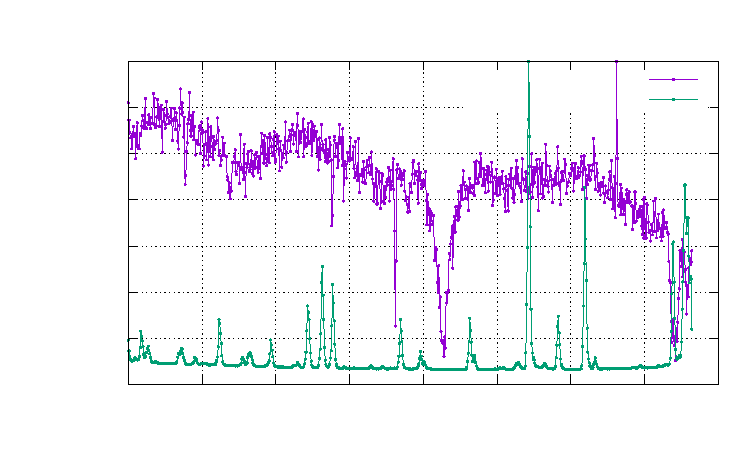
\includegraphics[width={360.00bp},height={216.00bp}]{60179-A1_data}}%
    \gplfronttext
  \end{picture}%
\endgroup
}
  \caption{}
\end{figure}
\begin{figure}[h]
  \centering
  \resizebox{.5\textwidth}{!}{% GNUPLOT: LaTeX picture with Postscript
\begingroup
  \makeatletter
  \providecommand\color[2][]{%
    \GenericError{(gnuplot) \space\space\space\@spaces}{%
      Package color not loaded in conjunction with
      terminal option `colourtext'%
    }{See the gnuplot documentation for explanation.%
    }{Either use 'blacktext' in gnuplot or load the package
      color.sty in LaTeX.}%
    \renewcommand\color[2][]{}%
  }%
  \providecommand\includegraphics[2][]{%
    \GenericError{(gnuplot) \space\space\space\@spaces}{%
      Package graphicx or graphics not loaded%
    }{See the gnuplot documentation for explanation.%
    }{The gnuplot epslatex terminal needs graphicx.sty or graphics.sty.}%
    \renewcommand\includegraphics[2][]{}%
  }%
  \providecommand\rotatebox[2]{#2}%
  \@ifundefined{ifGPcolor}{%
    \newif\ifGPcolor
    \GPcolortrue
  }{}%
  \@ifundefined{ifGPblacktext}{%
    \newif\ifGPblacktext
    \GPblacktexttrue
  }{}%
  % define a \g@addto@macro without @ in the name:
  \let\gplgaddtomacro\g@addto@macro
  % define empty templates for all commands taking text:
  \gdef\gplbacktext{}%
  \gdef\gplfronttext{}%
  \makeatother
  \ifGPblacktext
    % no textcolor at all
    \def\colorrgb#1{}%
    \def\colorgray#1{}%
  \else
    % gray or color?
    \ifGPcolor
      \def\colorrgb#1{\color[rgb]{#1}}%
      \def\colorgray#1{\color[gray]{#1}}%
      \expandafter\def\csname LTw\endcsname{\color{white}}%
      \expandafter\def\csname LTb\endcsname{\color{black}}%
      \expandafter\def\csname LTa\endcsname{\color{black}}%
      \expandafter\def\csname LT0\endcsname{\color[rgb]{1,0,0}}%
      \expandafter\def\csname LT1\endcsname{\color[rgb]{0,1,0}}%
      \expandafter\def\csname LT2\endcsname{\color[rgb]{0,0,1}}%
      \expandafter\def\csname LT3\endcsname{\color[rgb]{1,0,1}}%
      \expandafter\def\csname LT4\endcsname{\color[rgb]{0,1,1}}%
      \expandafter\def\csname LT5\endcsname{\color[rgb]{1,1,0}}%
      \expandafter\def\csname LT6\endcsname{\color[rgb]{0,0,0}}%
      \expandafter\def\csname LT7\endcsname{\color[rgb]{1,0.3,0}}%
      \expandafter\def\csname LT8\endcsname{\color[rgb]{0.5,0.5,0.5}}%
    \else
      % gray
      \def\colorrgb#1{\color{black}}%
      \def\colorgray#1{\color[gray]{#1}}%
      \expandafter\def\csname LTw\endcsname{\color{white}}%
      \expandafter\def\csname LTb\endcsname{\color{black}}%
      \expandafter\def\csname LTa\endcsname{\color{black}}%
      \expandafter\def\csname LT0\endcsname{\color{black}}%
      \expandafter\def\csname LT1\endcsname{\color{black}}%
      \expandafter\def\csname LT2\endcsname{\color{black}}%
      \expandafter\def\csname LT3\endcsname{\color{black}}%
      \expandafter\def\csname LT4\endcsname{\color{black}}%
      \expandafter\def\csname LT5\endcsname{\color{black}}%
      \expandafter\def\csname LT6\endcsname{\color{black}}%
      \expandafter\def\csname LT7\endcsname{\color{black}}%
      \expandafter\def\csname LT8\endcsname{\color{black}}%
    \fi
  \fi
    \setlength{\unitlength}{0.0500bp}%
    \ifx\gptboxheight\undefined%
      \newlength{\gptboxheight}%
      \newlength{\gptboxwidth}%
      \newsavebox{\gptboxtext}%
    \fi%
    \setlength{\fboxrule}{0.5pt}%
    \setlength{\fboxsep}{1pt}%
    \definecolor{tbcol}{rgb}{1,1,1}%
\begin{picture}(7200.00,4320.00)%
    \gplgaddtomacro\gplbacktext{%
      \csname LTb\endcsname%%
      \put(927,619){\makebox(0,0)[r]{\strut{}4\cdot10^{3}}}%
      \csname LTb\endcsname%%
      \put(927,1062){\makebox(0,0)[r]{\strut{}5\cdot10^{3}}}%
      \csname LTb\endcsname%%
      \put(927,1505){\makebox(0,0)[r]{\strut{}6\cdot10^{3}}}%
      \csname LTb\endcsname%%
      \put(927,1947){\makebox(0,0)[r]{\strut{}7\cdot10^{3}}}%
      \csname LTb\endcsname%%
      \put(927,2390){\makebox(0,0)[r]{\strut{}8\cdot10^{3}}}%
      \csname LTb\endcsname%%
      \put(927,2833){\makebox(0,0)[r]{\strut{}9\cdot10^{3}}}%
      \csname LTb\endcsname%%
      \put(927,3276){\makebox(0,0)[r]{\strut{}10\cdot10^{3}}}%
      \csname LTb\endcsname%%
      \put(927,3719){\makebox(0,0)[r]{\strut{}11\cdot10^{3}}}%
      \csname LTb\endcsname%%
      \put(2197,425){\makebox(0,0){\strut{}650\cdot10^{-9}}}%
      \csname LTb\endcsname%%
      \put(3662,425){\makebox(0,0){\strut{}655\cdot10^{-9}}}%
      \csname LTb\endcsname%%
      \put(5128,425){\makebox(0,0){\strut{}660\cdot10^{-9}}}%
      \csname LTb\endcsname%%
      \put(6593,425){\makebox(0,0){\strut{}665\cdot10^{-9}}}%
    }%
    \gplgaddtomacro\gplfronttext{%
      \csname LTb\endcsname%%
      \put(6123,986){\makebox(0,0)[r]{\strut{}Datenpunkte}}%
      \csname LTb\endcsname%%
      \put(6123,793){\makebox(0,0)[r]{\strut{}Anpassung $G_\text{f}(x)$}}%
      \csname LTb\endcsname%%
      \put(170,2169){\rotatebox{-270.00}{\makebox(0,0){\strut{}Amplitude$/\textrm{a.u.}$}}}%
      \csname LTb\endcsname%%
      \put(3955,135){\makebox(0,0){\strut{}Wellenlänge $\lambda/\SI{}{m}$}}%
      \csname LTb\endcsname%%
      \put(3955,4009){\makebox(0,0){\strut{}H$\alpha$(\SI{656}{nm})-Linie von 60179-A1 mit $\chi^2/\textrm{ddof}=\SI{2.32E-01}{}$}}%
    }%
    \gplbacktext
    \put(0,0){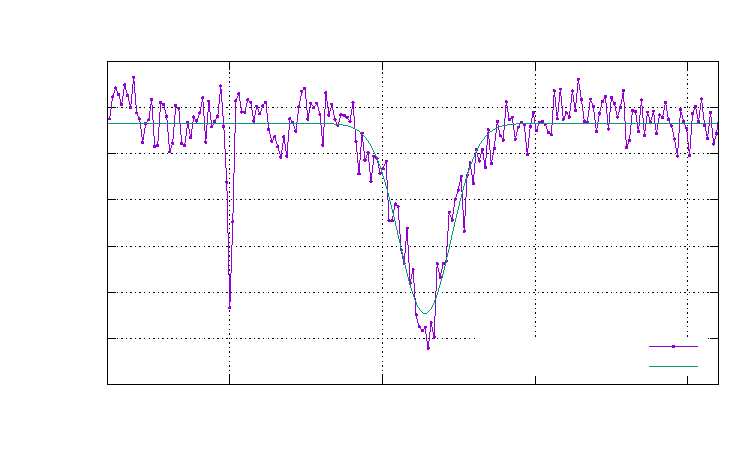
\includegraphics[width={360.00bp},height={216.00bp}]{60179-A1_gauss}}%
    \gplfronttext
  \end{picture}%
\endgroup
}
  \caption{}
\end{figure}
\begin{figure}[h]
  \centering
  \resizebox{.5\textwidth}{!}{% GNUPLOT: LaTeX picture with Postscript
\begingroup
  \makeatletter
  \providecommand\color[2][]{%
    \GenericError{(gnuplot) \space\space\space\@spaces}{%
      Package color not loaded in conjunction with
      terminal option `colourtext'%
    }{See the gnuplot documentation for explanation.%
    }{Either use 'blacktext' in gnuplot or load the package
      color.sty in LaTeX.}%
    \renewcommand\color[2][]{}%
  }%
  \providecommand\includegraphics[2][]{%
    \GenericError{(gnuplot) \space\space\space\@spaces}{%
      Package graphicx or graphics not loaded%
    }{See the gnuplot documentation for explanation.%
    }{The gnuplot epslatex terminal needs graphicx.sty or graphics.sty.}%
    \renewcommand\includegraphics[2][]{}%
  }%
  \providecommand\rotatebox[2]{#2}%
  \@ifundefined{ifGPcolor}{%
    \newif\ifGPcolor
    \GPcolortrue
  }{}%
  \@ifundefined{ifGPblacktext}{%
    \newif\ifGPblacktext
    \GPblacktexttrue
  }{}%
  % define a \g@addto@macro without @ in the name:
  \let\gplgaddtomacro\g@addto@macro
  % define empty templates for all commands taking text:
  \gdef\gplbacktext{}%
  \gdef\gplfronttext{}%
  \makeatother
  \ifGPblacktext
    % no textcolor at all
    \def\colorrgb#1{}%
    \def\colorgray#1{}%
  \else
    % gray or color?
    \ifGPcolor
      \def\colorrgb#1{\color[rgb]{#1}}%
      \def\colorgray#1{\color[gray]{#1}}%
      \expandafter\def\csname LTw\endcsname{\color{white}}%
      \expandafter\def\csname LTb\endcsname{\color{black}}%
      \expandafter\def\csname LTa\endcsname{\color{black}}%
      \expandafter\def\csname LT0\endcsname{\color[rgb]{1,0,0}}%
      \expandafter\def\csname LT1\endcsname{\color[rgb]{0,1,0}}%
      \expandafter\def\csname LT2\endcsname{\color[rgb]{0,0,1}}%
      \expandafter\def\csname LT3\endcsname{\color[rgb]{1,0,1}}%
      \expandafter\def\csname LT4\endcsname{\color[rgb]{0,1,1}}%
      \expandafter\def\csname LT5\endcsname{\color[rgb]{1,1,0}}%
      \expandafter\def\csname LT6\endcsname{\color[rgb]{0,0,0}}%
      \expandafter\def\csname LT7\endcsname{\color[rgb]{1,0.3,0}}%
      \expandafter\def\csname LT8\endcsname{\color[rgb]{0.5,0.5,0.5}}%
    \else
      % gray
      \def\colorrgb#1{\color{black}}%
      \def\colorgray#1{\color[gray]{#1}}%
      \expandafter\def\csname LTw\endcsname{\color{white}}%
      \expandafter\def\csname LTb\endcsname{\color{black}}%
      \expandafter\def\csname LTa\endcsname{\color{black}}%
      \expandafter\def\csname LT0\endcsname{\color{black}}%
      \expandafter\def\csname LT1\endcsname{\color{black}}%
      \expandafter\def\csname LT2\endcsname{\color{black}}%
      \expandafter\def\csname LT3\endcsname{\color{black}}%
      \expandafter\def\csname LT4\endcsname{\color{black}}%
      \expandafter\def\csname LT5\endcsname{\color{black}}%
      \expandafter\def\csname LT6\endcsname{\color{black}}%
      \expandafter\def\csname LT7\endcsname{\color{black}}%
      \expandafter\def\csname LT8\endcsname{\color{black}}%
    \fi
  \fi
    \setlength{\unitlength}{0.0500bp}%
    \ifx\gptboxheight\undefined%
      \newlength{\gptboxheight}%
      \newlength{\gptboxwidth}%
      \newsavebox{\gptboxtext}%
    \fi%
    \setlength{\fboxrule}{0.5pt}%
    \setlength{\fboxsep}{1pt}%
    \definecolor{tbcol}{rgb}{1,1,1}%
\begin{picture}(7200.00,4320.00)%
    \gplgaddtomacro\gplbacktext{%
      \csname LTb\endcsname%%
      \put(1123,619){\makebox(0,0)[r]{\strut{}$635\cdot10^{-9}$}}%
      \csname LTb\endcsname%%
      \put(1123,963){\makebox(0,0)[r]{\strut{}$640\cdot10^{-9}$}}%
      \csname LTb\endcsname%%
      \put(1123,1308){\makebox(0,0)[r]{\strut{}$645\cdot10^{-9}$}}%
      \csname LTb\endcsname%%
      \put(1123,1652){\makebox(0,0)[r]{\strut{}$650\cdot10^{-9}$}}%
      \csname LTb\endcsname%%
      \put(1123,1997){\makebox(0,0)[r]{\strut{}$655\cdot10^{-9}$}}%
      \csname LTb\endcsname%%
      \put(1123,2341){\makebox(0,0)[r]{\strut{}$660\cdot10^{-9}$}}%
      \csname LTb\endcsname%%
      \put(1123,2686){\makebox(0,0)[r]{\strut{}$665\cdot10^{-9}$}}%
      \csname LTb\endcsname%%
      \put(1123,3030){\makebox(0,0)[r]{\strut{}$670\cdot10^{-9}$}}%
      \csname LTb\endcsname%%
      \put(1123,3374){\makebox(0,0)[r]{\strut{}$675\cdot10^{-9}$}}%
      \csname LTb\endcsname%%
      \put(1123,3719){\makebox(0,0)[r]{\strut{}$680\cdot10^{-9}$}}%
      \csname LTb\endcsname%%
      \put(1221,425){\makebox(0,0){\strut{}$200$}}%
      \csname LTb\endcsname%%
      \put(1850,425){\makebox(0,0){\strut{}$250$}}%
      \csname LTb\endcsname%%
      \put(2480,425){\makebox(0,0){\strut{}$300$}}%
      \csname LTb\endcsname%%
      \put(3109,425){\makebox(0,0){\strut{}$350$}}%
      \csname LTb\endcsname%%
      \put(3739,425){\makebox(0,0){\strut{}$400$}}%
      \csname LTb\endcsname%%
      \put(4368,425){\makebox(0,0){\strut{}$450$}}%
      \csname LTb\endcsname%%
      \put(4997,425){\makebox(0,0){\strut{}$500$}}%
      \csname LTb\endcsname%%
      \put(5627,425){\makebox(0,0){\strut{}$550$}}%
      \csname LTb\endcsname%%
      \put(6256,425){\makebox(0,0){\strut{}$600$}}%
      \csname LTb\endcsname%%
      \put(6886,425){\makebox(0,0){\strut{}$650$}}%
    }%
    \gplgaddtomacro\gplfronttext{%
      \csname LTb\endcsname%%
      \put(170,2169){\rotatebox{-270}{\makebox(0,0){\strut{}Wellenlänge $\lambda/\SI{}{m}$}}}%
      \csname LTb\endcsname%%
      \put(4053,135){\makebox(0,0){\strut{}Pixelkoordinate$/\textrm{Pixel}$}}%
      \csname LTb\endcsname%%
      \put(6123,3545){\makebox(0,0)[r]{\strut{}Datenpunkte}}%
      \csname LTb\endcsname%%
      \put(6123,3351){\makebox(0,0)[r]{\strut{}Anpassung $\lambda_\text{f}(x)$}}%
      \csname LTb\endcsname%%
      \put(4053,4009){\makebox(0,0){\strut{}Kalibraiton des 60179-A1 Spektrums mit $\chi^2/\textrm{ddof}=\SI{1.45E-02}{}$}}%
    }%
    \gplbacktext
    \put(0,0){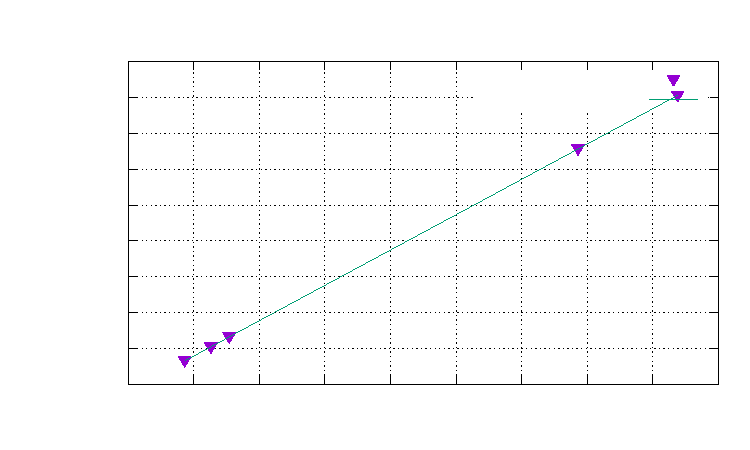
\includegraphics[width={360.00bp},height={216.00bp}]{60179-A1_kali}}%
    \gplfronttext
  \end{picture}%
\endgroup
}
  \caption{}
\end{figure}
\begin{figure}[h]
  \centering
  \resizebox{.5\textwidth}{!}{\input{äquivalenzbreiten.tex}}
  \caption{Äquivalenzbreiten}
\end{figure}
\begin{figure}[h]
  \centering
  \resizebox{.5\textwidth}{!}{% GNUPLOT: LaTeX picture with Postscript
\begingroup
  \makeatletter
  \providecommand\color[2][]{%
    \GenericError{(gnuplot) \space\space\space\@spaces}{%
      Package color not loaded in conjunction with
      terminal option `colourtext'%
    }{See the gnuplot documentation for explanation.%
    }{Either use 'blacktext' in gnuplot or load the package
      color.sty in LaTeX.}%
    \renewcommand\color[2][]{}%
  }%
  \providecommand\includegraphics[2][]{%
    \GenericError{(gnuplot) \space\space\space\@spaces}{%
      Package graphicx or graphics not loaded%
    }{See the gnuplot documentation for explanation.%
    }{The gnuplot epslatex terminal needs graphicx.sty or graphics.sty.}%
    \renewcommand\includegraphics[2][]{}%
  }%
  \providecommand\rotatebox[2]{#2}%
  \@ifundefined{ifGPcolor}{%
    \newif\ifGPcolor
    \GPcolortrue
  }{}%
  \@ifundefined{ifGPblacktext}{%
    \newif\ifGPblacktext
    \GPblacktexttrue
  }{}%
  % define a \g@addto@macro without @ in the name:
  \let\gplgaddtomacro\g@addto@macro
  % define empty templates for all commands taking text:
  \gdef\gplbacktext{}%
  \gdef\gplfronttext{}%
  \makeatother
  \ifGPblacktext
    % no textcolor at all
    \def\colorrgb#1{}%
    \def\colorgray#1{}%
  \else
    % gray or color?
    \ifGPcolor
      \def\colorrgb#1{\color[rgb]{#1}}%
      \def\colorgray#1{\color[gray]{#1}}%
      \expandafter\def\csname LTw\endcsname{\color{white}}%
      \expandafter\def\csname LTb\endcsname{\color{black}}%
      \expandafter\def\csname LTa\endcsname{\color{black}}%
      \expandafter\def\csname LT0\endcsname{\color[rgb]{1,0,0}}%
      \expandafter\def\csname LT1\endcsname{\color[rgb]{0,1,0}}%
      \expandafter\def\csname LT2\endcsname{\color[rgb]{0,0,1}}%
      \expandafter\def\csname LT3\endcsname{\color[rgb]{1,0,1}}%
      \expandafter\def\csname LT4\endcsname{\color[rgb]{0,1,1}}%
      \expandafter\def\csname LT5\endcsname{\color[rgb]{1,1,0}}%
      \expandafter\def\csname LT6\endcsname{\color[rgb]{0,0,0}}%
      \expandafter\def\csname LT7\endcsname{\color[rgb]{1,0.3,0}}%
      \expandafter\def\csname LT8\endcsname{\color[rgb]{0.5,0.5,0.5}}%
    \else
      % gray
      \def\colorrgb#1{\color{black}}%
      \def\colorgray#1{\color[gray]{#1}}%
      \expandafter\def\csname LTw\endcsname{\color{white}}%
      \expandafter\def\csname LTb\endcsname{\color{black}}%
      \expandafter\def\csname LTa\endcsname{\color{black}}%
      \expandafter\def\csname LT0\endcsname{\color{black}}%
      \expandafter\def\csname LT1\endcsname{\color{black}}%
      \expandafter\def\csname LT2\endcsname{\color{black}}%
      \expandafter\def\csname LT3\endcsname{\color{black}}%
      \expandafter\def\csname LT4\endcsname{\color{black}}%
      \expandafter\def\csname LT5\endcsname{\color{black}}%
      \expandafter\def\csname LT6\endcsname{\color{black}}%
      \expandafter\def\csname LT7\endcsname{\color{black}}%
      \expandafter\def\csname LT8\endcsname{\color{black}}%
    \fi
  \fi
    \setlength{\unitlength}{0.0500bp}%
    \ifx\gptboxheight\undefined%
      \newlength{\gptboxheight}%
      \newlength{\gptboxwidth}%
      \newsavebox{\gptboxtext}%
    \fi%
    \setlength{\fboxrule}{0.5pt}%
    \setlength{\fboxsep}{1pt}%
    \definecolor{tbcol}{rgb}{1,1,1}%
\begin{picture}(7200.00,4320.00)%
    \gplgaddtomacro\gplbacktext{%
      \csname LTb\endcsname%%
      \put(927,619){\makebox(0,0)[r]{\strut{}36\cdot10^{3}}}%
      \csname LTb\endcsname%%
      \put(927,1135){\makebox(0,0)[r]{\strut{}38\cdot10^{3}}}%
      \csname LTb\endcsname%%
      \put(927,1652){\makebox(0,0)[r]{\strut{}40\cdot10^{3}}}%
      \csname LTb\endcsname%%
      \put(927,2169){\makebox(0,0)[r]{\strut{}42\cdot10^{3}}}%
      \csname LTb\endcsname%%
      \put(927,2686){\makebox(0,0)[r]{\strut{}44\cdot10^{3}}}%
      \csname LTb\endcsname%%
      \put(927,3202){\makebox(0,0)[r]{\strut{}46\cdot10^{3}}}%
      \csname LTb\endcsname%%
      \put(927,3719){\makebox(0,0)[r]{\strut{}48\cdot10^{3}}}%
      \csname LTb\endcsname%%
      \put(2127,425){\makebox(0,0){\strut{}647\cdot10^{-9}}}%
      \csname LTb\endcsname%%
      \put(3641,425){\makebox(0,0){\strut{}648\cdot10^{-9}}}%
      \csname LTb\endcsname%%
      \put(5155,425){\makebox(0,0){\strut{}649\cdot10^{-9}}}%
      \csname LTb\endcsname%%
      \put(6669,425){\makebox(0,0){\strut{}650\cdot10^{-9}}}%
    }%
    \gplgaddtomacro\gplfronttext{%
      \csname LTb\endcsname%%
      \put(6123,3545){\makebox(0,0)[r]{\strut{}Datenpunkte}}%
      \csname LTb\endcsname%%
      \put(6123,3351){\makebox(0,0)[r]{\strut{}Anpassung $G_\text{f}(x)$}}%
      \csname LTb\endcsname%%
      \put(170,2169){\rotatebox{-270.00}{\makebox(0,0){\strut{}Amplitude$/\textrm{a.u.}$}}}%
      \csname LTb\endcsname%%
      \put(3955,135){\makebox(0,0){\strut{}Wellenlänge $\lambda/\SI{}{m}$}}%
      \csname LTb\endcsname%%
      \put(3955,4009){\makebox(0,0){\strut{}H$\alpha$(\SI{656}{nm})-Linie von He2 mit $\chi^2/\textrm{ddof}=\SI{2.02E-01}{}$}}%
    }%
    \gplbacktext
    \put(0,0){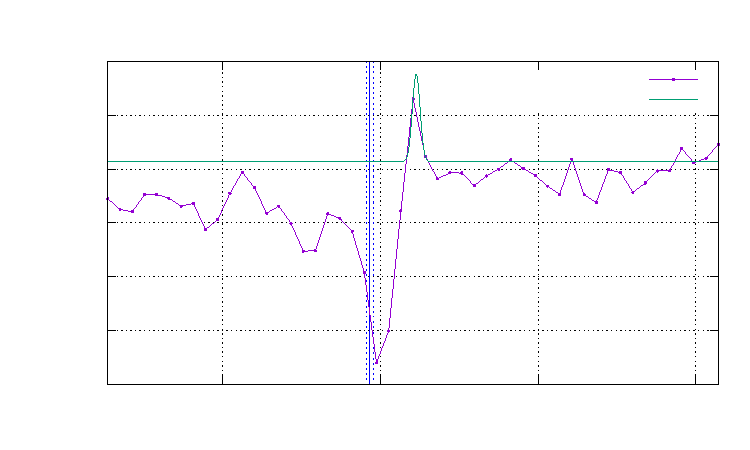
\includegraphics[width={360.00bp},height={216.00bp}]{P-Cygni_He2_gauss}}%
    \gplfronttext
  \end{picture}%
\endgroup
}
  \caption{}
\end{figure}
\begin{figure}[h]
  \centering
  \resizebox{.5\textwidth}{!}{% GNUPLOT: LaTeX picture with Postscript
\begingroup
  \makeatletter
  \providecommand\color[2][]{%
    \GenericError{(gnuplot) \space\space\space\@spaces}{%
      Package color not loaded in conjunction with
      terminal option `colourtext'%
    }{See the gnuplot documentation for explanation.%
    }{Either use 'blacktext' in gnuplot or load the package
      color.sty in LaTeX.}%
    \renewcommand\color[2][]{}%
  }%
  \providecommand\includegraphics[2][]{%
    \GenericError{(gnuplot) \space\space\space\@spaces}{%
      Package graphicx or graphics not loaded%
    }{See the gnuplot documentation for explanation.%
    }{The gnuplot epslatex terminal needs graphicx.sty or graphics.sty.}%
    \renewcommand\includegraphics[2][]{}%
  }%
  \providecommand\rotatebox[2]{#2}%
  \@ifundefined{ifGPcolor}{%
    \newif\ifGPcolor
    \GPcolortrue
  }{}%
  \@ifundefined{ifGPblacktext}{%
    \newif\ifGPblacktext
    \GPblacktexttrue
  }{}%
  % define a \g@addto@macro without @ in the name:
  \let\gplgaddtomacro\g@addto@macro
  % define empty templates for all commands taking text:
  \gdef\gplbacktext{}%
  \gdef\gplfronttext{}%
  \makeatother
  \ifGPblacktext
    % no textcolor at all
    \def\colorrgb#1{}%
    \def\colorgray#1{}%
  \else
    % gray or color?
    \ifGPcolor
      \def\colorrgb#1{\color[rgb]{#1}}%
      \def\colorgray#1{\color[gray]{#1}}%
      \expandafter\def\csname LTw\endcsname{\color{white}}%
      \expandafter\def\csname LTb\endcsname{\color{black}}%
      \expandafter\def\csname LTa\endcsname{\color{black}}%
      \expandafter\def\csname LT0\endcsname{\color[rgb]{1,0,0}}%
      \expandafter\def\csname LT1\endcsname{\color[rgb]{0,1,0}}%
      \expandafter\def\csname LT2\endcsname{\color[rgb]{0,0,1}}%
      \expandafter\def\csname LT3\endcsname{\color[rgb]{1,0,1}}%
      \expandafter\def\csname LT4\endcsname{\color[rgb]{0,1,1}}%
      \expandafter\def\csname LT5\endcsname{\color[rgb]{1,1,0}}%
      \expandafter\def\csname LT6\endcsname{\color[rgb]{0,0,0}}%
      \expandafter\def\csname LT7\endcsname{\color[rgb]{1,0.3,0}}%
      \expandafter\def\csname LT8\endcsname{\color[rgb]{0.5,0.5,0.5}}%
    \else
      % gray
      \def\colorrgb#1{\color{black}}%
      \def\colorgray#1{\color[gray]{#1}}%
      \expandafter\def\csname LTw\endcsname{\color{white}}%
      \expandafter\def\csname LTb\endcsname{\color{black}}%
      \expandafter\def\csname LTa\endcsname{\color{black}}%
      \expandafter\def\csname LT0\endcsname{\color{black}}%
      \expandafter\def\csname LT1\endcsname{\color{black}}%
      \expandafter\def\csname LT2\endcsname{\color{black}}%
      \expandafter\def\csname LT3\endcsname{\color{black}}%
      \expandafter\def\csname LT4\endcsname{\color{black}}%
      \expandafter\def\csname LT5\endcsname{\color{black}}%
      \expandafter\def\csname LT6\endcsname{\color{black}}%
      \expandafter\def\csname LT7\endcsname{\color{black}}%
      \expandafter\def\csname LT8\endcsname{\color{black}}%
    \fi
  \fi
    \setlength{\unitlength}{0.0500bp}%
    \ifx\gptboxheight\undefined%
      \newlength{\gptboxheight}%
      \newlength{\gptboxwidth}%
      \newsavebox{\gptboxtext}%
    \fi%
    \setlength{\fboxrule}{0.5pt}%
    \setlength{\fboxsep}{1pt}%
    \definecolor{tbcol}{rgb}{1,1,1}%
\begin{picture}(7200.00,4320.00)%
    \gplgaddtomacro\gplbacktext{%
      \csname LTb\endcsname%%
      \put(1025,619){\makebox(0,0)[r]{\strut{}$0\cdot10^{0}$}}%
      \csname LTb\endcsname%%
      \put(1025,929){\makebox(0,0)[r]{\strut{}$100\cdot10^{3}$}}%
      \csname LTb\endcsname%%
      \put(1025,1239){\makebox(0,0)[r]{\strut{}$200\cdot10^{3}$}}%
      \csname LTb\endcsname%%
      \put(1025,1549){\makebox(0,0)[r]{\strut{}$300\cdot10^{3}$}}%
      \csname LTb\endcsname%%
      \put(1025,1859){\makebox(0,0)[r]{\strut{}$400\cdot10^{3}$}}%
      \csname LTb\endcsname%%
      \put(1025,2169){\makebox(0,0)[r]{\strut{}$500\cdot10^{3}$}}%
      \csname LTb\endcsname%%
      \put(1025,2479){\makebox(0,0)[r]{\strut{}$600\cdot10^{3}$}}%
      \csname LTb\endcsname%%
      \put(1025,2789){\makebox(0,0)[r]{\strut{}$700\cdot10^{3}$}}%
      \csname LTb\endcsname%%
      \put(1025,3099){\makebox(0,0)[r]{\strut{}$800\cdot10^{3}$}}%
      \csname LTb\endcsname%%
      \put(1025,3409){\makebox(0,0)[r]{\strut{}$900\cdot10^{3}$}}%
      \csname LTb\endcsname%%
      \put(1025,3719){\makebox(0,0)[r]{\strut{}$1\cdot10^{6}$}}%
      \csname LTb\endcsname%%
      \put(1891,425){\makebox(0,0){\strut{}$649\cdot10^{-9}$}}%
      \csname LTb\endcsname%%
      \put(2759,425){\makebox(0,0){\strut{}$652\cdot10^{-9}$}}%
      \csname LTb\endcsname%%
      \put(3628,425){\makebox(0,0){\strut{}$655\cdot10^{-9}$}}%
      \csname LTb\endcsname%%
      \put(4497,425){\makebox(0,0){\strut{}$658\cdot10^{-9}$}}%
      \csname LTb\endcsname%%
      \put(5366,425){\makebox(0,0){\strut{}$661\cdot10^{-9}$}}%
      \csname LTb\endcsname%%
      \put(6235,425){\makebox(0,0){\strut{}$664\cdot10^{-9}$}}%
    }%
    \gplgaddtomacro\gplfronttext{%
      \csname LTb\endcsname%%
      \put(170,2169){\rotatebox{-270}{\makebox(0,0){\strut{}Amplitude$/\textrm{a.u.}$}}}%
      \csname LTb\endcsname%%
      \put(4004,135){\makebox(0,0){\strut{}Wellenlänge $\lambda/\SI{}{m}$}}%
      \csname LTb\endcsname%%
      \put(6123,3545){\makebox(0,0)[r]{\strut{}Datenpunkte}}%
      \csname LTb\endcsname%%
      \put(6123,3351){\makebox(0,0)[r]{\strut{}Anpassung $G_\text{f}(x)$}}%
      \csname LTb\endcsname%%
      \put(4004,4009){\makebox(0,0){\strut{}Spektrallinie von H mit $\chi^2/\textrm{ddof}=\SI{1.50E+01}{}$}}%
    }%
    \gplbacktext
    \put(0,0){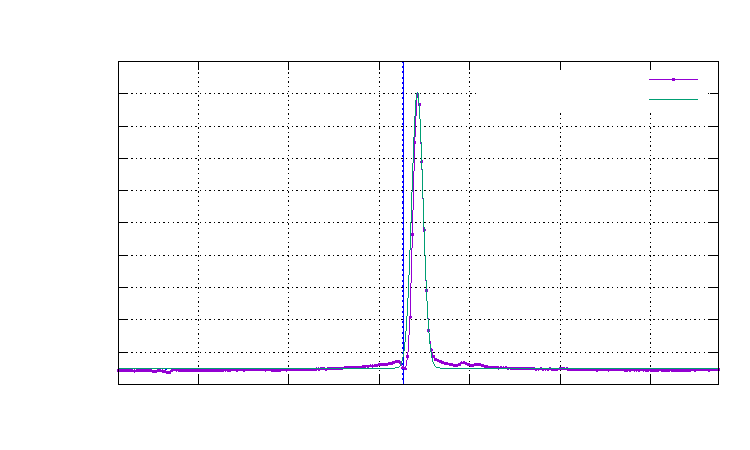
\includegraphics[width={360.00bp},height={216.00bp}]{P-Cygni_H_gauss}}%
    \gplfronttext
  \end{picture}%
\endgroup
}
  \caption{}
\end{figure}
\begin{figure}[h]
  \centering
  \resizebox{.5\textwidth}{!}{% GNUPLOT: LaTeX picture with Postscript
\begingroup
  \makeatletter
  \providecommand\color[2][]{%
    \GenericError{(gnuplot) \space\space\space\@spaces}{%
      Package color not loaded in conjunction with
      terminal option `colourtext'%
    }{See the gnuplot documentation for explanation.%
    }{Either use 'blacktext' in gnuplot or load the package
      color.sty in LaTeX.}%
    \renewcommand\color[2][]{}%
  }%
  \providecommand\includegraphics[2][]{%
    \GenericError{(gnuplot) \space\space\space\@spaces}{%
      Package graphicx or graphics not loaded%
    }{See the gnuplot documentation for explanation.%
    }{The gnuplot epslatex terminal needs graphicx.sty or graphics.sty.}%
    \renewcommand\includegraphics[2][]{}%
  }%
  \providecommand\rotatebox[2]{#2}%
  \@ifundefined{ifGPcolor}{%
    \newif\ifGPcolor
    \GPcolortrue
  }{}%
  \@ifundefined{ifGPblacktext}{%
    \newif\ifGPblacktext
    \GPblacktexttrue
  }{}%
  % define a \g@addto@macro without @ in the name:
  \let\gplgaddtomacro\g@addto@macro
  % define empty templates for all commands taking text:
  \gdef\gplbacktext{}%
  \gdef\gplfronttext{}%
  \makeatother
  \ifGPblacktext
    % no textcolor at all
    \def\colorrgb#1{}%
    \def\colorgray#1{}%
  \else
    % gray or color?
    \ifGPcolor
      \def\colorrgb#1{\color[rgb]{#1}}%
      \def\colorgray#1{\color[gray]{#1}}%
      \expandafter\def\csname LTw\endcsname{\color{white}}%
      \expandafter\def\csname LTb\endcsname{\color{black}}%
      \expandafter\def\csname LTa\endcsname{\color{black}}%
      \expandafter\def\csname LT0\endcsname{\color[rgb]{1,0,0}}%
      \expandafter\def\csname LT1\endcsname{\color[rgb]{0,1,0}}%
      \expandafter\def\csname LT2\endcsname{\color[rgb]{0,0,1}}%
      \expandafter\def\csname LT3\endcsname{\color[rgb]{1,0,1}}%
      \expandafter\def\csname LT4\endcsname{\color[rgb]{0,1,1}}%
      \expandafter\def\csname LT5\endcsname{\color[rgb]{1,1,0}}%
      \expandafter\def\csname LT6\endcsname{\color[rgb]{0,0,0}}%
      \expandafter\def\csname LT7\endcsname{\color[rgb]{1,0.3,0}}%
      \expandafter\def\csname LT8\endcsname{\color[rgb]{0.5,0.5,0.5}}%
    \else
      % gray
      \def\colorrgb#1{\color{black}}%
      \def\colorgray#1{\color[gray]{#1}}%
      \expandafter\def\csname LTw\endcsname{\color{white}}%
      \expandafter\def\csname LTb\endcsname{\color{black}}%
      \expandafter\def\csname LTa\endcsname{\color{black}}%
      \expandafter\def\csname LT0\endcsname{\color{black}}%
      \expandafter\def\csname LT1\endcsname{\color{black}}%
      \expandafter\def\csname LT2\endcsname{\color{black}}%
      \expandafter\def\csname LT3\endcsname{\color{black}}%
      \expandafter\def\csname LT4\endcsname{\color{black}}%
      \expandafter\def\csname LT5\endcsname{\color{black}}%
      \expandafter\def\csname LT6\endcsname{\color{black}}%
      \expandafter\def\csname LT7\endcsname{\color{black}}%
      \expandafter\def\csname LT8\endcsname{\color{black}}%
    \fi
  \fi
    \setlength{\unitlength}{0.0500bp}%
    \ifx\gptboxheight\undefined%
      \newlength{\gptboxheight}%
      \newlength{\gptboxwidth}%
      \newsavebox{\gptboxtext}%
    \fi%
    \setlength{\fboxrule}{0.5pt}%
    \setlength{\fboxsep}{1pt}%
    \definecolor{tbcol}{rgb}{1,1,1}%
\begin{picture}(7200.00,4320.00)%
    \gplgaddtomacro\gplbacktext{%
      \csname LTb\endcsname%%
      \put(1025,619){\makebox(0,0)[r]{\strut{}$30\cdot10^{3}$}}%
      \csname LTb\endcsname%%
      \put(1025,1006){\makebox(0,0)[r]{\strut{}$40\cdot10^{3}$}}%
      \csname LTb\endcsname%%
      \put(1025,1394){\makebox(0,0)[r]{\strut{}$50\cdot10^{3}$}}%
      \csname LTb\endcsname%%
      \put(1025,1781){\makebox(0,0)[r]{\strut{}$60\cdot10^{3}$}}%
      \csname LTb\endcsname%%
      \put(1025,2169){\makebox(0,0)[r]{\strut{}$70\cdot10^{3}$}}%
      \csname LTb\endcsname%%
      \put(1025,2556){\makebox(0,0)[r]{\strut{}$80\cdot10^{3}$}}%
      \csname LTb\endcsname%%
      \put(1025,2944){\makebox(0,0)[r]{\strut{}$90\cdot10^{3}$}}%
      \csname LTb\endcsname%%
      \put(1025,3331){\makebox(0,0)[r]{\strut{}$100\cdot10^{3}$}}%
      \csname LTb\endcsname%%
      \put(1025,3719){\makebox(0,0)[r]{\strut{}$110\cdot10^{3}$}}%
      \csname LTb\endcsname%%
      \put(1326,425){\makebox(0,0){\strut{}$666\cdot10^{-9}$}}%
      \csname LTb\endcsname%%
      \put(2786,425){\makebox(0,0){\strut{}$667\cdot10^{-9}$}}%
      \csname LTb\endcsname%%
      \put(4245,425){\makebox(0,0){\strut{}$668\cdot10^{-9}$}}%
      \csname LTb\endcsname%%
      \put(5705,425){\makebox(0,0){\strut{}$669\cdot10^{-9}$}}%
    }%
    \gplgaddtomacro\gplfronttext{%
      \csname LTb\endcsname%%
      \put(170,2169){\rotatebox{-270}{\makebox(0,0){\strut{}Amplitude$/\textrm{a.u.}$}}}%
      \csname LTb\endcsname%%
      \put(4004,135){\makebox(0,0){\strut{}Wellenlänge $\lambda/\SI{}{m}$}}%
      \csname LTb\endcsname%%
      \put(6123,3545){\makebox(0,0)[r]{\strut{}Datenpunkte}}%
      \csname LTb\endcsname%%
      \put(6123,3351){\makebox(0,0)[r]{\strut{}Anpassung $G_\text{f}(x)$}}%
      \csname LTb\endcsname%%
      \put(4004,4009){\makebox(0,0){\strut{}Spektrallinie von N2 mit $\chi^2/\textrm{ddof}=\SI{2.17E-01}{}$}}%
    }%
    \gplbacktext
    \put(0,0){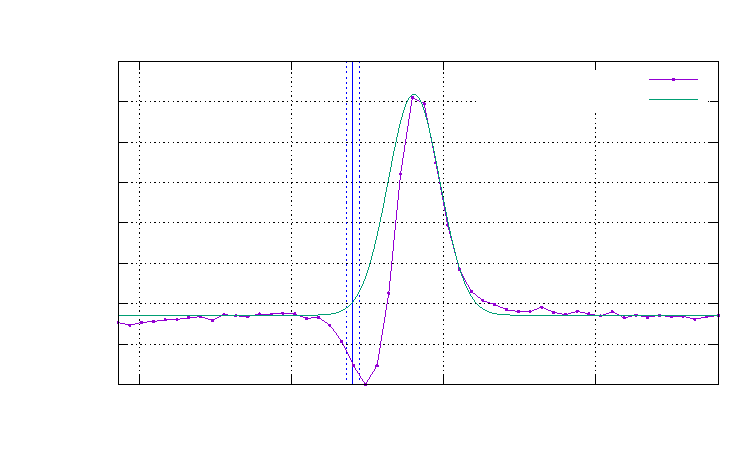
\includegraphics[width={360.00bp},height={216.00bp}]{P-Cygni_N2_gauss}}%
    \gplfronttext
  \end{picture}%
\endgroup
}
  \caption{}
\end{figure}
\begin{figure}[h]
  \centering
  \resizebox{.5\textwidth}{!}{% GNUPLOT: LaTeX picture with Postscript
\begingroup
  \makeatletter
  \providecommand\color[2][]{%
    \GenericError{(gnuplot) \space\space\space\@spaces}{%
      Package color not loaded in conjunction with
      terminal option `colourtext'%
    }{See the gnuplot documentation for explanation.%
    }{Either use 'blacktext' in gnuplot or load the package
      color.sty in LaTeX.}%
    \renewcommand\color[2][]{}%
  }%
  \providecommand\includegraphics[2][]{%
    \GenericError{(gnuplot) \space\space\space\@spaces}{%
      Package graphicx or graphics not loaded%
    }{See the gnuplot documentation for explanation.%
    }{The gnuplot epslatex terminal needs graphicx.sty or graphics.sty.}%
    \renewcommand\includegraphics[2][]{}%
  }%
  \providecommand\rotatebox[2]{#2}%
  \@ifundefined{ifGPcolor}{%
    \newif\ifGPcolor
    \GPcolortrue
  }{}%
  \@ifundefined{ifGPblacktext}{%
    \newif\ifGPblacktext
    \GPblacktexttrue
  }{}%
  % define a \g@addto@macro without @ in the name:
  \let\gplgaddtomacro\g@addto@macro
  % define empty templates for all commands taking text:
  \gdef\gplbacktext{}%
  \gdef\gplfronttext{}%
  \makeatother
  \ifGPblacktext
    % no textcolor at all
    \def\colorrgb#1{}%
    \def\colorgray#1{}%
  \else
    % gray or color?
    \ifGPcolor
      \def\colorrgb#1{\color[rgb]{#1}}%
      \def\colorgray#1{\color[gray]{#1}}%
      \expandafter\def\csname LTw\endcsname{\color{white}}%
      \expandafter\def\csname LTb\endcsname{\color{black}}%
      \expandafter\def\csname LTa\endcsname{\color{black}}%
      \expandafter\def\csname LT0\endcsname{\color[rgb]{1,0,0}}%
      \expandafter\def\csname LT1\endcsname{\color[rgb]{0,1,0}}%
      \expandafter\def\csname LT2\endcsname{\color[rgb]{0,0,1}}%
      \expandafter\def\csname LT3\endcsname{\color[rgb]{1,0,1}}%
      \expandafter\def\csname LT4\endcsname{\color[rgb]{0,1,1}}%
      \expandafter\def\csname LT5\endcsname{\color[rgb]{1,1,0}}%
      \expandafter\def\csname LT6\endcsname{\color[rgb]{0,0,0}}%
      \expandafter\def\csname LT7\endcsname{\color[rgb]{1,0.3,0}}%
      \expandafter\def\csname LT8\endcsname{\color[rgb]{0.5,0.5,0.5}}%
    \else
      % gray
      \def\colorrgb#1{\color{black}}%
      \def\colorgray#1{\color[gray]{#1}}%
      \expandafter\def\csname LTw\endcsname{\color{white}}%
      \expandafter\def\csname LTb\endcsname{\color{black}}%
      \expandafter\def\csname LTa\endcsname{\color{black}}%
      \expandafter\def\csname LT0\endcsname{\color{black}}%
      \expandafter\def\csname LT1\endcsname{\color{black}}%
      \expandafter\def\csname LT2\endcsname{\color{black}}%
      \expandafter\def\csname LT3\endcsname{\color{black}}%
      \expandafter\def\csname LT4\endcsname{\color{black}}%
      \expandafter\def\csname LT5\endcsname{\color{black}}%
      \expandafter\def\csname LT6\endcsname{\color{black}}%
      \expandafter\def\csname LT7\endcsname{\color{black}}%
      \expandafter\def\csname LT8\endcsname{\color{black}}%
    \fi
  \fi
    \setlength{\unitlength}{0.0500bp}%
    \ifx\gptboxheight\undefined%
      \newlength{\gptboxheight}%
      \newlength{\gptboxwidth}%
      \newsavebox{\gptboxtext}%
    \fi%
    \setlength{\fboxrule}{0.5pt}%
    \setlength{\fboxsep}{1pt}%
    \definecolor{tbcol}{rgb}{1,1,1}%
\begin{picture}(7200.00,4320.00)%
    \gplgaddtomacro\gplbacktext{%
      \csname LTb\endcsname%%
      \put(927,619){\makebox(0,0)[r]{\strut{}$40\cdot10^{3}$}}%
      \csname LTb\endcsname%%
      \put(927,963){\makebox(0,0)[r]{\strut{}$42\cdot10^{3}$}}%
      \csname LTb\endcsname%%
      \put(927,1308){\makebox(0,0)[r]{\strut{}$44\cdot10^{3}$}}%
      \csname LTb\endcsname%%
      \put(927,1652){\makebox(0,0)[r]{\strut{}$46\cdot10^{3}$}}%
      \csname LTb\endcsname%%
      \put(927,1997){\makebox(0,0)[r]{\strut{}$48\cdot10^{3}$}}%
      \csname LTb\endcsname%%
      \put(927,2341){\makebox(0,0)[r]{\strut{}$50\cdot10^{3}$}}%
      \csname LTb\endcsname%%
      \put(927,2686){\makebox(0,0)[r]{\strut{}$52\cdot10^{3}$}}%
      \csname LTb\endcsname%%
      \put(927,3030){\makebox(0,0)[r]{\strut{}$54\cdot10^{3}$}}%
      \csname LTb\endcsname%%
      \put(927,3374){\makebox(0,0)[r]{\strut{}$56\cdot10^{3}$}}%
      \csname LTb\endcsname%%
      \put(927,3719){\makebox(0,0)[r]{\strut{}$58\cdot10^{3}$}}%
      \csname LTb\endcsname%%
      \put(1025,425){\makebox(0,0){\strut{}$632\cdot10^{-9}$}}%
      \csname LTb\endcsname%%
      \put(1758,425){\makebox(0,0){\strut{}$633\cdot10^{-9}$}}%
      \csname LTb\endcsname%%
      \put(2490,425){\makebox(0,0){\strut{}$634\cdot10^{-9}$}}%
      \csname LTb\endcsname%%
      \put(3223,425){\makebox(0,0){\strut{}$635\cdot10^{-9}$}}%
      \csname LTb\endcsname%%
      \put(3955,425){\makebox(0,0){\strut{}$636\cdot10^{-9}$}}%
      \csname LTb\endcsname%%
      \put(4688,425){\makebox(0,0){\strut{}$637\cdot10^{-9}$}}%
      \csname LTb\endcsname%%
      \put(5421,425){\makebox(0,0){\strut{}$638\cdot10^{-9}$}}%
      \csname LTb\endcsname%%
      \put(6153,425){\makebox(0,0){\strut{}$639\cdot10^{-9}$}}%
      \csname LTb\endcsname%%
      \put(6886,425){\makebox(0,0){\strut{}$640\cdot10^{-9}$}}%
    }%
    \gplgaddtomacro\gplfronttext{%
      \csname LTb\endcsname%%
      \put(170,2169){\rotatebox{-270}{\makebox(0,0){\strut{}Amplitude$/\textrm{a.u.}$}}}%
      \csname LTb\endcsname%%
      \put(3955,135){\makebox(0,0){\strut{}Wellenlänge $\lambda/\SI{}{m}$}}%
      \csname LTb\endcsname%%
      \put(6123,3545){\makebox(0,0)[r]{\strut{}Datenpunkte}}%
      \csname LTb\endcsname%%
      \put(6123,3351){\makebox(0,0)[r]{\strut{}Anpassung $G_\text{f}(x)$}}%
      \csname LTb\endcsname%%
      \put(3955,4009){\makebox(0,0){\strut{}Doublet von Si3 mit $\chi^2/\textrm{ddof}=\SI{5.51E-01}{}$}}%
    }%
    \gplbacktext
    \put(0,0){\includegraphics[width={360.00bp},height={216.00bp}]{P-Cygni_Si3_doublet}}%
    \gplfronttext
  \end{picture}%
\endgroup
}
  \caption{}
\end{figure}
\begin{figure}[h]
  \centering
  \resizebox{.5\textwidth}{!}{% GNUPLOT: LaTeX picture with Postscript
\begingroup
  \makeatletter
  \providecommand\color[2][]{%
    \GenericError{(gnuplot) \space\space\space\@spaces}{%
      Package color not loaded in conjunction with
      terminal option `colourtext'%
    }{See the gnuplot documentation for explanation.%
    }{Either use 'blacktext' in gnuplot or load the package
      color.sty in LaTeX.}%
    \renewcommand\color[2][]{}%
  }%
  \providecommand\includegraphics[2][]{%
    \GenericError{(gnuplot) \space\space\space\@spaces}{%
      Package graphicx or graphics not loaded%
    }{See the gnuplot documentation for explanation.%
    }{The gnuplot epslatex terminal needs graphicx.sty or graphics.sty.}%
    \renewcommand\includegraphics[2][]{}%
  }%
  \providecommand\rotatebox[2]{#2}%
  \@ifundefined{ifGPcolor}{%
    \newif\ifGPcolor
    \GPcolortrue
  }{}%
  \@ifundefined{ifGPblacktext}{%
    \newif\ifGPblacktext
    \GPblacktexttrue
  }{}%
  % define a \g@addto@macro without @ in the name:
  \let\gplgaddtomacro\g@addto@macro
  % define empty templates for all commands taking text:
  \gdef\gplbacktext{}%
  \gdef\gplfronttext{}%
  \makeatother
  \ifGPblacktext
    % no textcolor at all
    \def\colorrgb#1{}%
    \def\colorgray#1{}%
  \else
    % gray or color?
    \ifGPcolor
      \def\colorrgb#1{\color[rgb]{#1}}%
      \def\colorgray#1{\color[gray]{#1}}%
      \expandafter\def\csname LTw\endcsname{\color{white}}%
      \expandafter\def\csname LTb\endcsname{\color{black}}%
      \expandafter\def\csname LTa\endcsname{\color{black}}%
      \expandafter\def\csname LT0\endcsname{\color[rgb]{1,0,0}}%
      \expandafter\def\csname LT1\endcsname{\color[rgb]{0,1,0}}%
      \expandafter\def\csname LT2\endcsname{\color[rgb]{0,0,1}}%
      \expandafter\def\csname LT3\endcsname{\color[rgb]{1,0,1}}%
      \expandafter\def\csname LT4\endcsname{\color[rgb]{0,1,1}}%
      \expandafter\def\csname LT5\endcsname{\color[rgb]{1,1,0}}%
      \expandafter\def\csname LT6\endcsname{\color[rgb]{0,0,0}}%
      \expandafter\def\csname LT7\endcsname{\color[rgb]{1,0.3,0}}%
      \expandafter\def\csname LT8\endcsname{\color[rgb]{0.5,0.5,0.5}}%
    \else
      % gray
      \def\colorrgb#1{\color{black}}%
      \def\colorgray#1{\color[gray]{#1}}%
      \expandafter\def\csname LTw\endcsname{\color{white}}%
      \expandafter\def\csname LTb\endcsname{\color{black}}%
      \expandafter\def\csname LTa\endcsname{\color{black}}%
      \expandafter\def\csname LT0\endcsname{\color{black}}%
      \expandafter\def\csname LT1\endcsname{\color{black}}%
      \expandafter\def\csname LT2\endcsname{\color{black}}%
      \expandafter\def\csname LT3\endcsname{\color{black}}%
      \expandafter\def\csname LT4\endcsname{\color{black}}%
      \expandafter\def\csname LT5\endcsname{\color{black}}%
      \expandafter\def\csname LT6\endcsname{\color{black}}%
      \expandafter\def\csname LT7\endcsname{\color{black}}%
      \expandafter\def\csname LT8\endcsname{\color{black}}%
    \fi
  \fi
    \setlength{\unitlength}{0.0500bp}%
    \ifx\gptboxheight\undefined%
      \newlength{\gptboxheight}%
      \newlength{\gptboxwidth}%
      \newsavebox{\gptboxtext}%
    \fi%
    \setlength{\fboxrule}{0.5pt}%
    \setlength{\fboxsep}{1pt}%
    \definecolor{tbcol}{rgb}{1,1,1}%
\begin{picture}(7200.00,4320.00)%
    \gplgaddtomacro\gplbacktext{%
      \csname LTb\endcsname%%
      \put(1025,619){\makebox(0,0)[r]{\strut{}0\cdot10^{0}}}%
      \csname LTb\endcsname%%
      \put(1025,963){\makebox(0,0)[r]{\strut{}100\cdot10^{3}}}%
      \csname LTb\endcsname%%
      \put(1025,1308){\makebox(0,0)[r]{\strut{}200\cdot10^{3}}}%
      \csname LTb\endcsname%%
      \put(1025,1652){\makebox(0,0)[r]{\strut{}300\cdot10^{3}}}%
      \csname LTb\endcsname%%
      \put(1025,1997){\makebox(0,0)[r]{\strut{}400\cdot10^{3}}}%
      \csname LTb\endcsname%%
      \put(1025,2341){\makebox(0,0)[r]{\strut{}500\cdot10^{3}}}%
      \csname LTb\endcsname%%
      \put(1025,2686){\makebox(0,0)[r]{\strut{}600\cdot10^{3}}}%
      \csname LTb\endcsname%%
      \put(1025,3030){\makebox(0,0)[r]{\strut{}700\cdot10^{3}}}%
      \csname LTb\endcsname%%
      \put(1025,3374){\makebox(0,0)[r]{\strut{}800\cdot10^{3}}}%
      \csname LTb\endcsname%%
      \put(1025,3719){\makebox(0,0)[r]{\strut{}900\cdot10^{3}}}%
      \csname LTb\endcsname%%
      \put(1123,425){\makebox(0,0){\strut{}630\cdot10^{-9}}}%
      \csname LTb\endcsname%%
      \put(2084,425){\makebox(0,0){\strut{}640\cdot10^{-9}}}%
      \csname LTb\endcsname%%
      \put(3044,425){\makebox(0,0){\strut{}650\cdot10^{-9}}}%
      \csname LTb\endcsname%%
      \put(4004,425){\makebox(0,0){\strut{}660\cdot10^{-9}}}%
      \csname LTb\endcsname%%
      \put(4965,425){\makebox(0,0){\strut{}670\cdot10^{-9}}}%
      \csname LTb\endcsname%%
      \put(5925,425){\makebox(0,0){\strut{}680\cdot10^{-9}}}%
      \csname LTb\endcsname%%
      \put(6886,425){\makebox(0,0){\strut{}690\cdot10^{-9}}}%
    }%
    \gplgaddtomacro\gplfronttext{%
      \csname LTb\endcsname%%
      \put(6123,3545){\makebox(0,0)[r]{\strut{}Datenpunkte}}%
      \csname LTb\endcsname%%
      \put(170,2169){\rotatebox{-270.00}{\makebox(0,0){\strut{}Amplitude$/\SI{}{a.u}$}}}%
      \csname LTb\endcsname%%
      \put(4004,135){\makebox(0,0){\strut{}Wellenlänge $\lambda/\SI{}{m}$}}%
      \csname LTb\endcsname%%
      \put(4004,4009){\makebox(0,0){\strut{}P-Cygni Spektrum}}%
    }%
    \gplbacktext
    \put(0,0){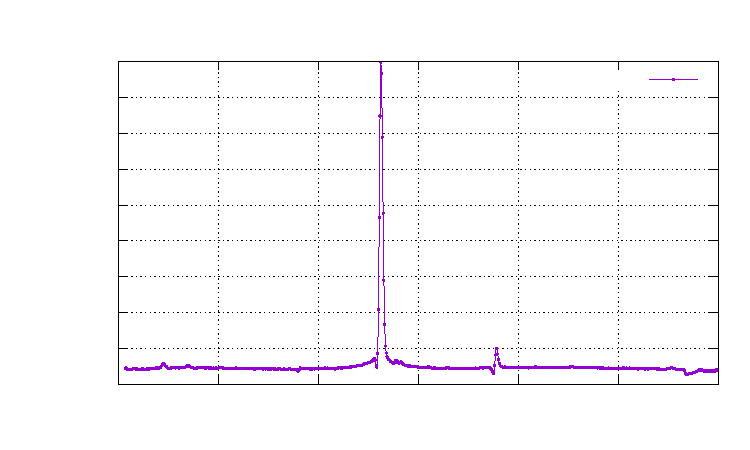
\includegraphics[width={360.00bp},height={216.00bp}]{P_Cygni_spectra}}%
    \gplfronttext
  \end{picture}%
\endgroup
}
  \caption{}
\end{figure}
